\chapter{Neutrino experiments}
\label{c:expIntro}

\section{Introduction}
Since the discovery of the neutrino in 1956 by Reines and Cowan~\cite{6Reines} a multitude of neutrino experiments have tried to measure the properties of the different neutrino flavours. Since the Homestake experiment, many other experiments have been run to measure neutrino oscillations and the mass of neutrinos. A detailed description of these experiments is outside of the scope of this thesis, however in this section a description of the main types of experiments and milestones will be presented.

Neutrino experiments are split into four different categories based on their primary neutrino source. Each type features its own advantages and issues.
The experiment types are those that detect:
\begin{itemize}
\item Atmospheric neutrinos
\item Solar neutrinos
\item Accelerator neutrinos
\item Reactor neutrinos.
\end{itemize}
Each will be described briefly before examples are given.

\pagebreak
\newpage
\section{Atmospheric neutrino experiments}

As mentioned in section~\ref{subsection:Missing} neutrinos at low energy ranges ($<18$ MeV) are produced through nuclear interactions in stars. There are other cosmological phenomena which produce neutrinos, and some searches are looking for signs of new physics in these signals. 

The Earth is constantly bombarded by cosmic-ray particles from space. When they hit the atmosphere, these high-energy protons interact with air molecules to produce showers of pions, which subsequently decay to muons and muon-neutrinos. This process is similar to that used to produce neutrino beams from particle accelerators. Early observations of atmospheric neutrinos were contradictory, with some experiments observing approximately the expected ratio while others saw significantly fewer muon-neutrinos than expected, similar to the missing solar neutrinos. This became known as the Atmospheric Neutrino Anomaly. This was a measurement performed by Super-Kamiokande and confirmed, together with the Homestake experiment, the existence of neutrino oscillations~\cite{10Fukuda, 9Davis}.

The atmospheric neutrinos are produced from cosmic-rays interacting through nuclear interactions producing pions which decay into muons, electrons and neutrinos through the following interactions:
\begin{align}
\pi^{\pm} &\rightarrow \mu^{\pm}  \nu_\mu (\bar{\nu_\mu}) \\
\mu^{\pm} &\rightarrow e^{\pm} \bar{\nu_e}  \nu_\mu  (\nu_e \bar{\nu_\mu}).
\end{align}

The neutrinos produced have an energy that can be in the GeV to PeV range. However, it is impossible to control the source and difficult to get many events due to the low fluxes expected from cosmic rays. 

Looking at the two flavour oscillation formula:
\begin{equation}
P_{\nu_\mu \rightarrow \nu_y} (L) = \sin^2(2\theta_{\mu y})\sin^2 \frac{[1.27\Delta m_{\mu y}^2 L]}{E_\nu}
%\label{eq:twoPNeutrinoosc}
\end{equation}

these experiments are able to measure the direction angle ($\theta$), to extract the distance the neutrino has travelled $L$, and the energy ($E_\nu$) of the neutrino to extract the mixing angle $\theta_{\mu y}$ and the mass-squared difference $\Delta m^2_{\mu y}$. Given the current experimental values, these experiments are best suited to look for $\theta_{23}$ and $|\Delta m_{32}^2 |$.

%these experiments are looking for a specific $\theta$ for a given $\Delta m^2$ in the two oscillation formula.  Starting with $\nu_\mu$ going to $\tau$ or $e$ as $P_{\nu_\mu \rightarrow \nu_x} = \sin^2(2\theta)\sin^2 \frac{1.27\Delta m^2 D}{E_\nu}$ with $\theta$ the mixing angle between states, $\delta m^2$ the difference of the neutrino masses squared, D is the distance from the creation point (km) and $E_\nu$  the energy of the neutrino in GeV. Given the current experimental values, these experiments are best suited to look for $\theta_23$ and $|\Delta m_{32}^2 |$.

%\textbf{why best? Mentioned above in theory? Mention best values and different hierarchy?}

\if{0}
\textbf{Mixed answer}
For these experiments either solar, or other cosmological sources are used to provide the neutrinos. The main advantages are that the energy can be very high, GeV to PeV range, and it is possible to use the earth to remove all background providing an extremely clean signal. However, it is impossible to control the source and difficult to get many events due to the low fluxes expected from astrophysical objects. 
\fi

%In most cases the detectors are based on detecting Cerenkov light being emitted in a medium. Cerenkov light is emitted when a particle travels faster than the speed of light inside a medium. This creates a shock wave similar to the sonic boom that is visible in nuclear reactors as a bluish light.


\subsection{Historical experiments}
In the beginning of the 1960s the Kolar Gold Fields (KGF) experiment, in a mine near Kolar (India), was the first experiment to record atmospheric neutrinos by detecting inelastic neutrino events in the large amount of rock covering the experiment producing two distinct muon tracks through charge current interactions $\nu + N \rightarrow N' + \mu $~\cite{96Achar}. These results were used to estimate the neutrino induced muon interaction flux. %It was also the first usage of a Cherenkov detector. Cerenkov light is emitted when a particle travels faster than the speed of light inside a medium. This creates a shock wave similar to the sonic boom that is visible in nuclear reactors as a bluish light.

At the same time a similar experiment in the E.R.P. Mines in South Africa reproduced the results and improved some of the measurements~\cite{97Reines}.

\subsection{NUSEX}
The NUSEX detector, installed in the Mont Blanc tunnel, collected data between June 1982 and 1988 and was a cube 3.5 m$^3$ consisting of 134 iron plates with plastic streamer tubes interlaced between the different iron plates providing 150 tons of instrumented mass (see ~\FigRef{fig:nusex}). One of the main results from NUSEX was that they did not observe any difference in the rate of electron and muon neutrinos as seen in \FigRef{fig:nusexres}, in contradiction with the Kamiokande experiment~\cite{56NUSEX, 57NUSEX}.

\begin{figure}[h!]
\centering
  \centering
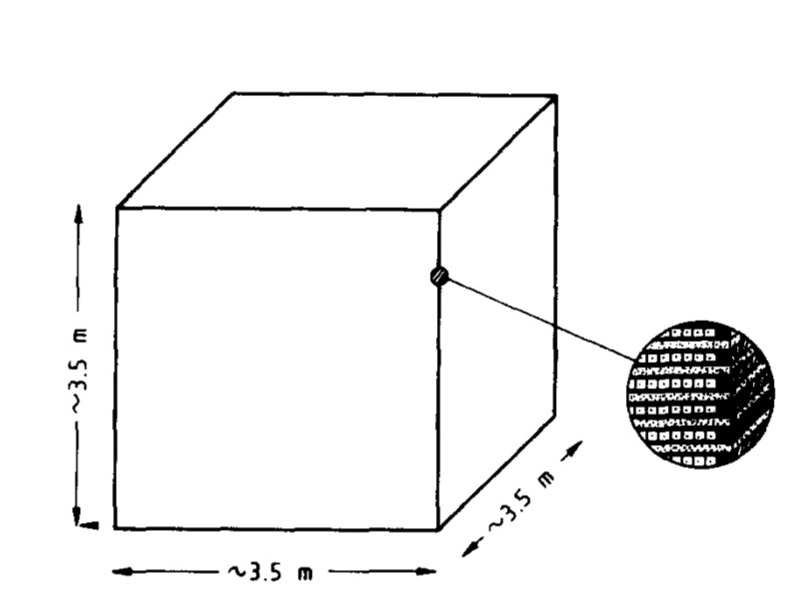
\includegraphics[width=0.49\textwidth]{figures/nusex1.jpeg}
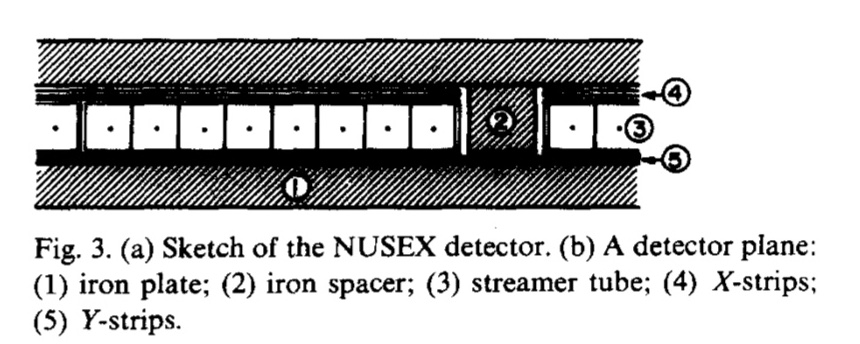
\includegraphics[width=0.49\textwidth]{figures/nusex2.jpeg}
\vspace{2mm}
\caption{A sketch of the NUSEX detector with various parts highlighted~\cite{56NUSEX}.}
\label{fig:nusex}
\end{figure}

\begin{figure}[h!]
\centering
  \centering
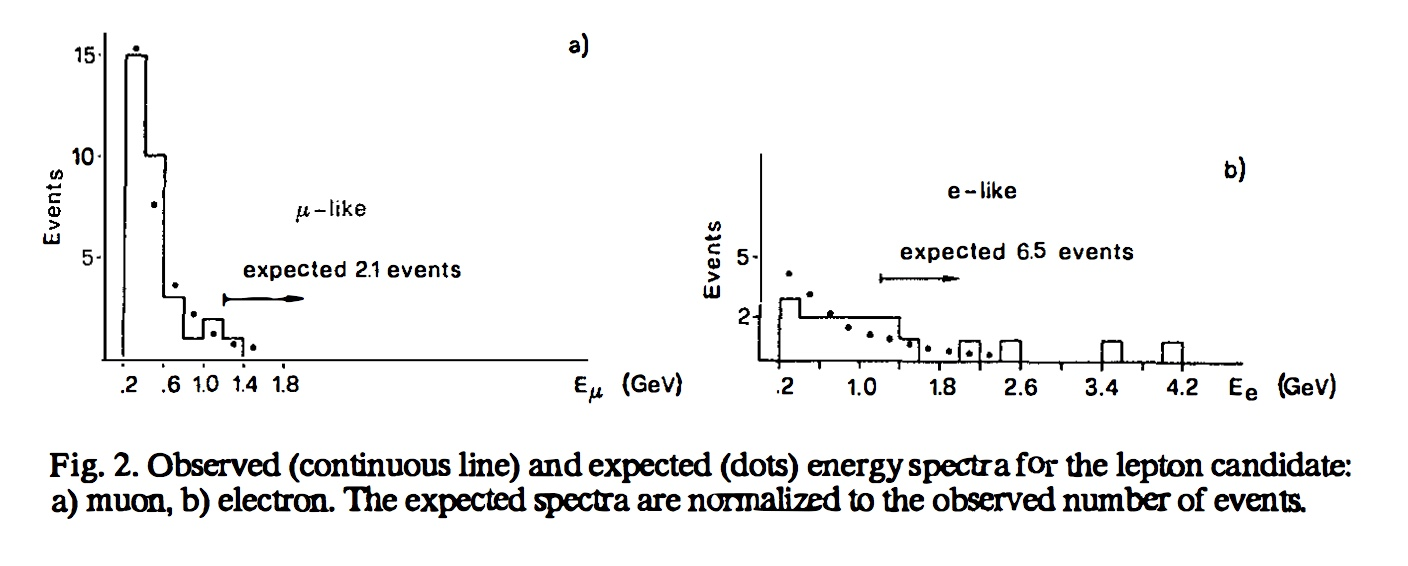
\includegraphics[width=0.9\textwidth]{figures/nusexres.jpeg}
\vspace{2mm}
\caption{Data compared to Monte Carlo for 50 neutrino events in the NUSEX detector and showing consistency within errors~\cite{57NUSEX}.}
\label{fig:nusexres}
\end{figure}

\subsection{KamiokaNDE}
The Kamioka Nucleon Decay Experiment (KamiokaNDE) was a 3000 ton water Cherenkov detector installed in the Kamioka mine in Japan, 1000 m under the top of a mountain (\FigRef{fig:Kam}). The goal of the detector, which began operation in 1983, was to study and search for nucleon decay. Cherenkov light is emitted when a particle travels faster than the speed of light inside a medium. This creates a shock wave similar to the sonic boom that is visible in nuclear reactors as a bluish light. In KamiokaNDE the Cherenkov light was detected using 1000 large PhotoMultiplier Tubes (PMTs)~\cite{58KAMIOKA}.


\if{0}
 In Japan, the Kamiokande detector (1983-1996, 3 kiloton) and Super-Kamiokande (in operation since 1996, 50 kiloton) have achieved several important scientific results, notably detection of extraterrestrial neutrinos from the Sun [40] and Supernova 1987a [41, 42], and discovery of neutrino flavor mixing and neutrino mass [6, 43]. In the K2K long baseline neutrino oscillation experiment, Super-K and a one kiloton water Cherenkov detector (1KT) provided indis- pensable data on the neutrino beam flux and its energy spectrum at the neutrino production site (using 1KT) and a location 250 km farther away (using Super-K) [22]. Super-K again is playing the role of the far detector in the ongoing T2K experiment which reported an indication of %νμ → νe oscillations in June 2011 [1].
Good paper for all of this! %https://arxiv.org/pdf/1109.3262.pdf
6, Y. Fukuda et al. (Super-Kamiokande), Phys. Rev. Lett. 81, 1562 (1998), arXiv:hep-ex/9807003.
40, K. S. Hirata et al. (KAMIOKANDE-II), Phys. Rev. Lett. 63, 16 (1989).
41, K. Hirata et al. (KAMIOKANDE-II), Phys. Rev. Lett. 58, 1490 (1987).
42, K. S. Hirata et al. (KAMIOKANDE-II), Phys. Rev. D38, 448 (1988).
43, S. Fukuda et al. (Super-Kamiokande), Phys. Lett. B539, 179 (2002), arXiv:hep-ex/0205075
Kamiokande2 was solar?
\fi
\begin{figure}[h!]
\centering
  \centering
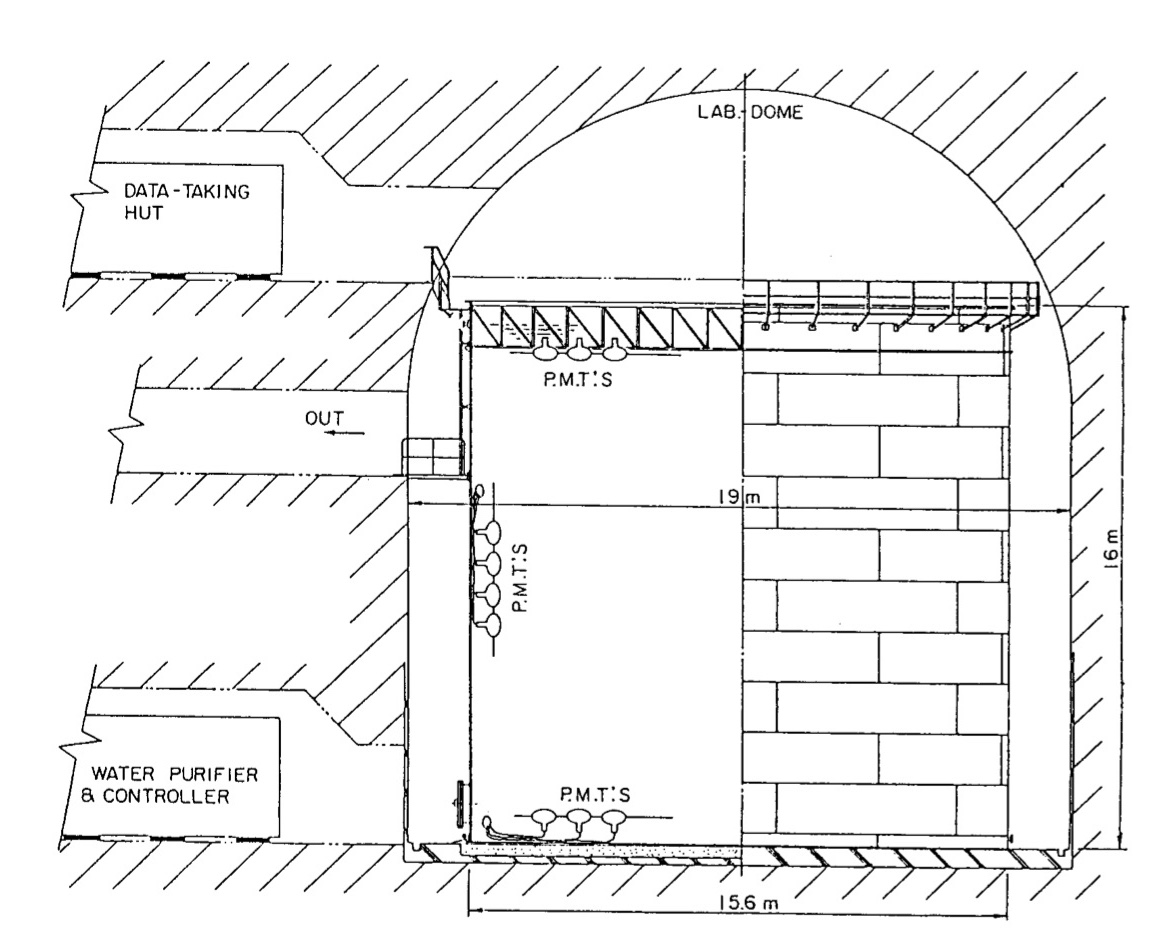
\includegraphics[width=0.9\textwidth]{figures/Kamioka1.jpeg}
\vspace{2mm}
\caption{Schematic image of the KamiokaNDE detector.~\cite{58KAMIOKA}.}
\label{fig:Kam}
\end{figure}

\begin{figure}[h!]
\centering
  \centering
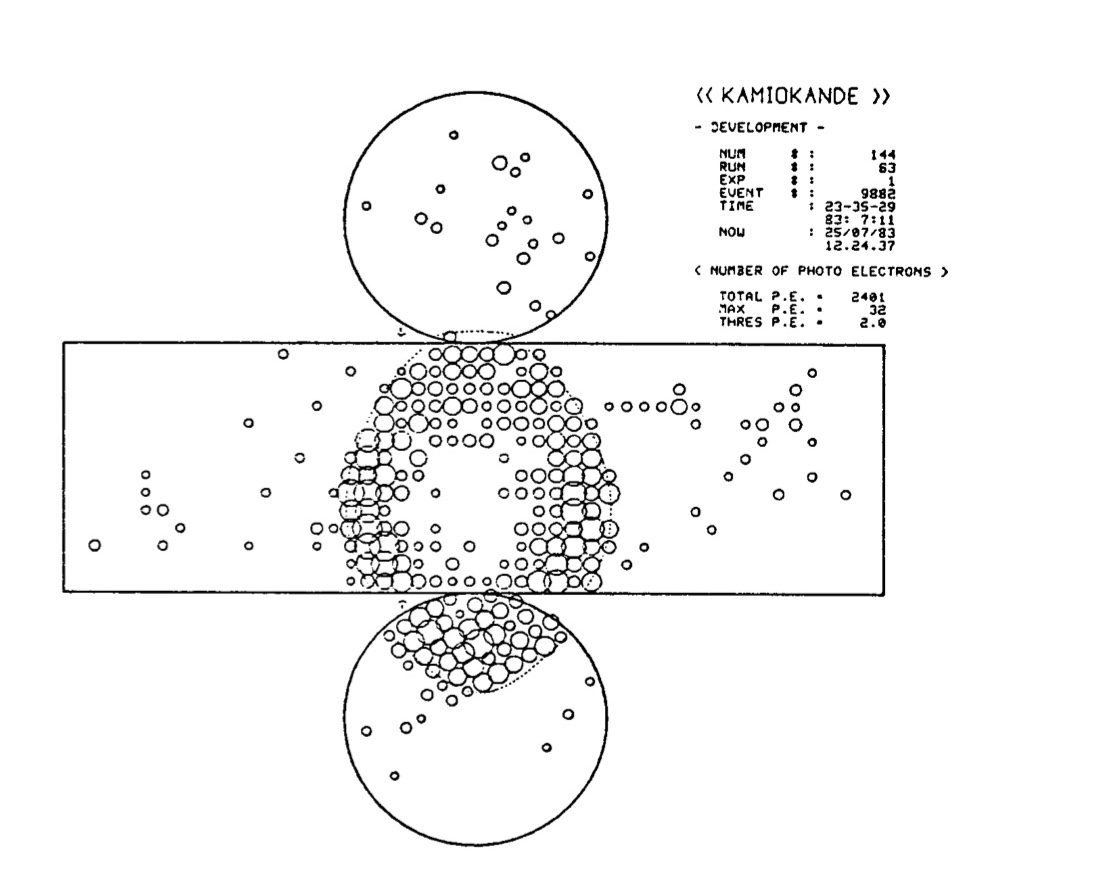
\includegraphics[width=0.49\textwidth]{figures/Kamioka2.jpeg}
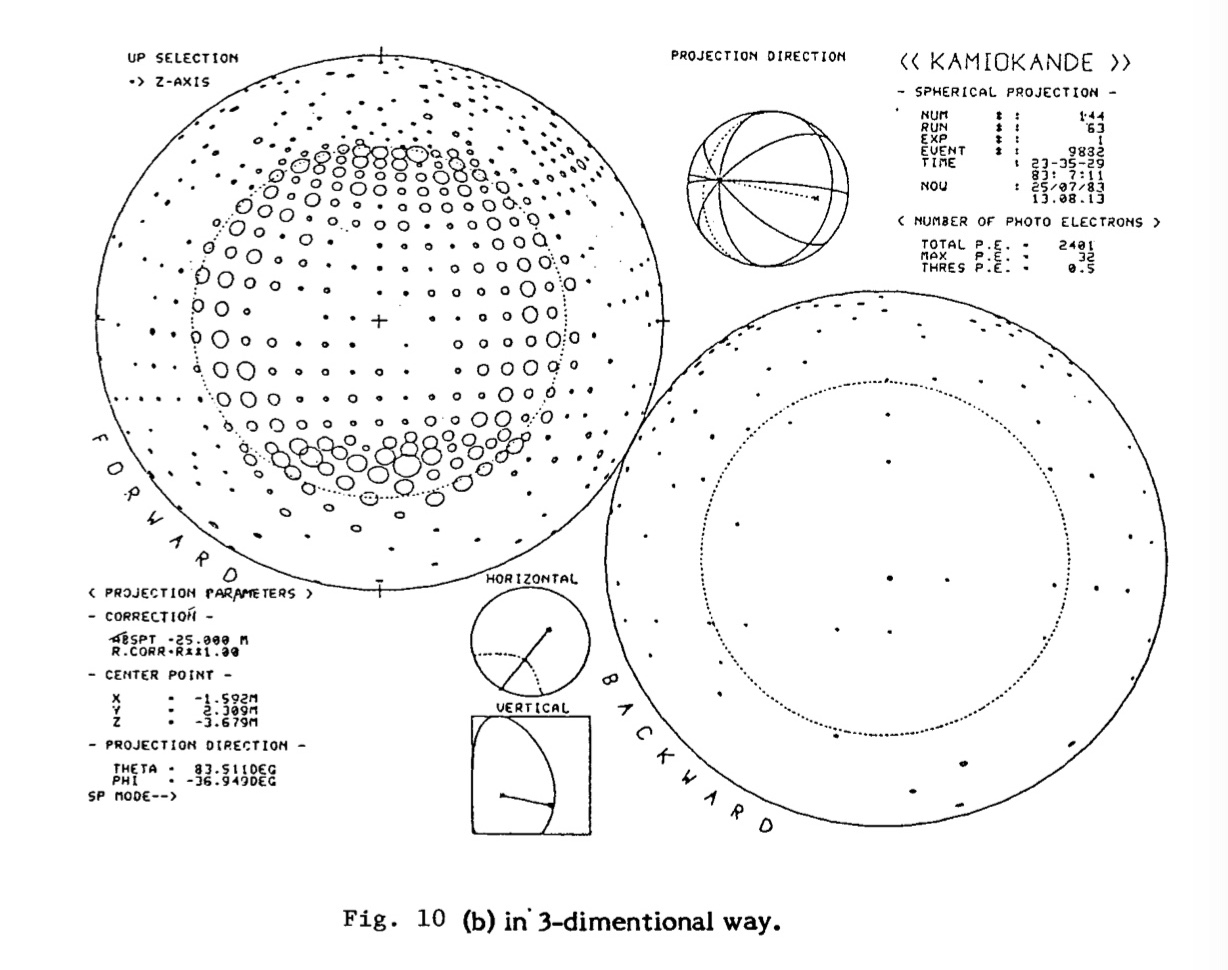
\includegraphics[width=0.49\textwidth]{figures/Kamioka3.jpeg}
\vspace{2mm}
\caption{A sample event showing Cherenkov rings in KamiokaNDE produced by a muon event~\cite{58KAMIOKA}.}
\label{fig:Kam2}
\end{figure}
KamiokaNDE found an anomaly between the expected number of $\nu_\mu$ and $\nu_e$ atmospheric neutrinos, which was the first hint that possibly atmospheric neutrinos were oscillating (figures~\ref{fig:Kam2} and~\ref{fig:Kam3}.
%The main result was finding a slight discrepancy between data and simulations, seen in~\FigRef{fig:Kam3}, hinting at at a possibility that atmospheric neutrinos were oscillating.
\begin{figure}[h!]
\centering
  \centering
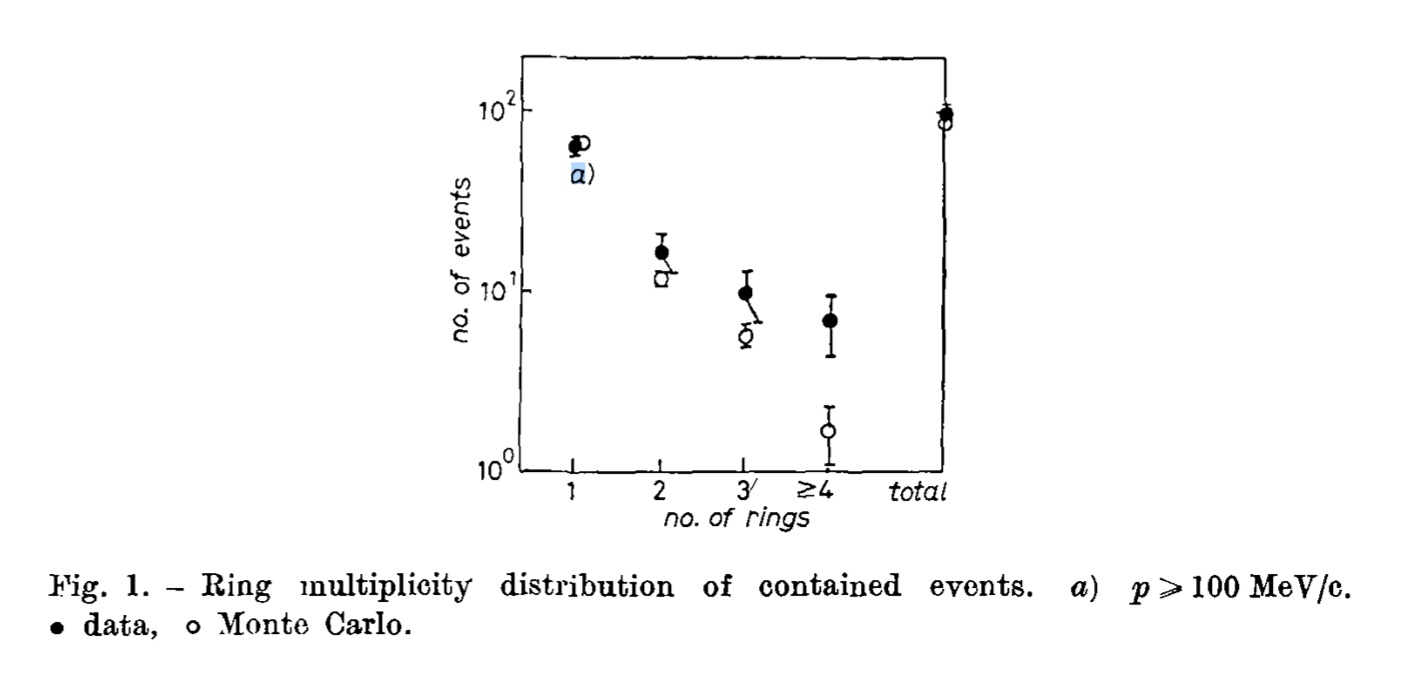
\includegraphics[width=0.49\textwidth]{figures/Kamioka4.jpeg}
\vspace{2mm}
\caption{Comparing ring multiplicity distributions between data (black) and simulations (white) in KamiokaNDE~\cite{59KAMIOKA}.}
\label{fig:Kam3}
\end{figure}

\subsection{IMB}
The Irvine- Michigan-Brookhaven (IMB) groups built a 8 kiloton water Cherenkov detector 600 m under the Morton Salt Mine in Cleveland which began data taking in 1986. The design was similar to KamiokaNDE and also observed the anomaly between $\nu_\mu$ and $\nu_e$ atmospheric neutrino rates~\cite{60IMB}.


\subsection{Super-KamiokaNDE}~\label{subsection:Super-K}
Super-KamiokaNDE (Super-K)~\cite{20SUPERK}, a water Cherenkov detector located 1 km underground also in the Kamioka mine in Japan and began operations in 1996. The detector consists of a cylindrical stainless steel tank holding 50 ktons of ultra-pure water (\FigRef{fig:SK}. Super-K performed the first experimental observation that the neutrino has non-zero mass~\cite{10Fukuda} and also managed to detect strong evidence of muon neutrino oscillation to tau neutrinos from the analysis of atmospheric neutrinos interacting in the water target (see~\FigRef{fig:SK2}). The deviation from unity is evidence for the discovery of neutrino oscillations and the lines show the expected shape for oscillation from muon neutrinos to tau neutrinos~\cite{10Fukuda}. It also shows that electron-like events have no significant variation in length over neutrino energy whereby muon-like events are about half of the expected rate at large values of length over neutrino energy.
%where at large length over neutrino energy muon-like events have come to close to half of the initial rate.

\begin{figure}[h!]
\centering
  \centering
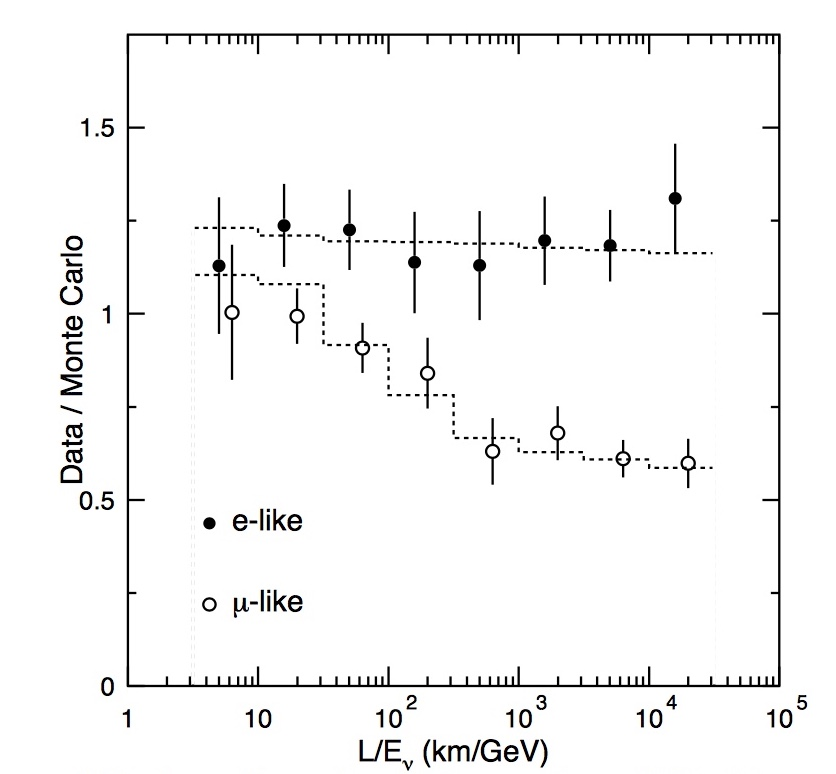
\includegraphics[width=0.49\textwidth]{figures/simuSK2.jpeg}
\vspace{2mm}
\caption{Comparison of the ratio of data vs Monte Carlo vs length over neutrino energy for fully contained atmospheric electron-like and muon-like events in the Super-K detector~\cite{10Fukuda}.}
\label{fig:SK2}
\end{figure}

\begin{figure}[h!]
\centering
\begin{subfigure}{.5\textwidth}
  \centering
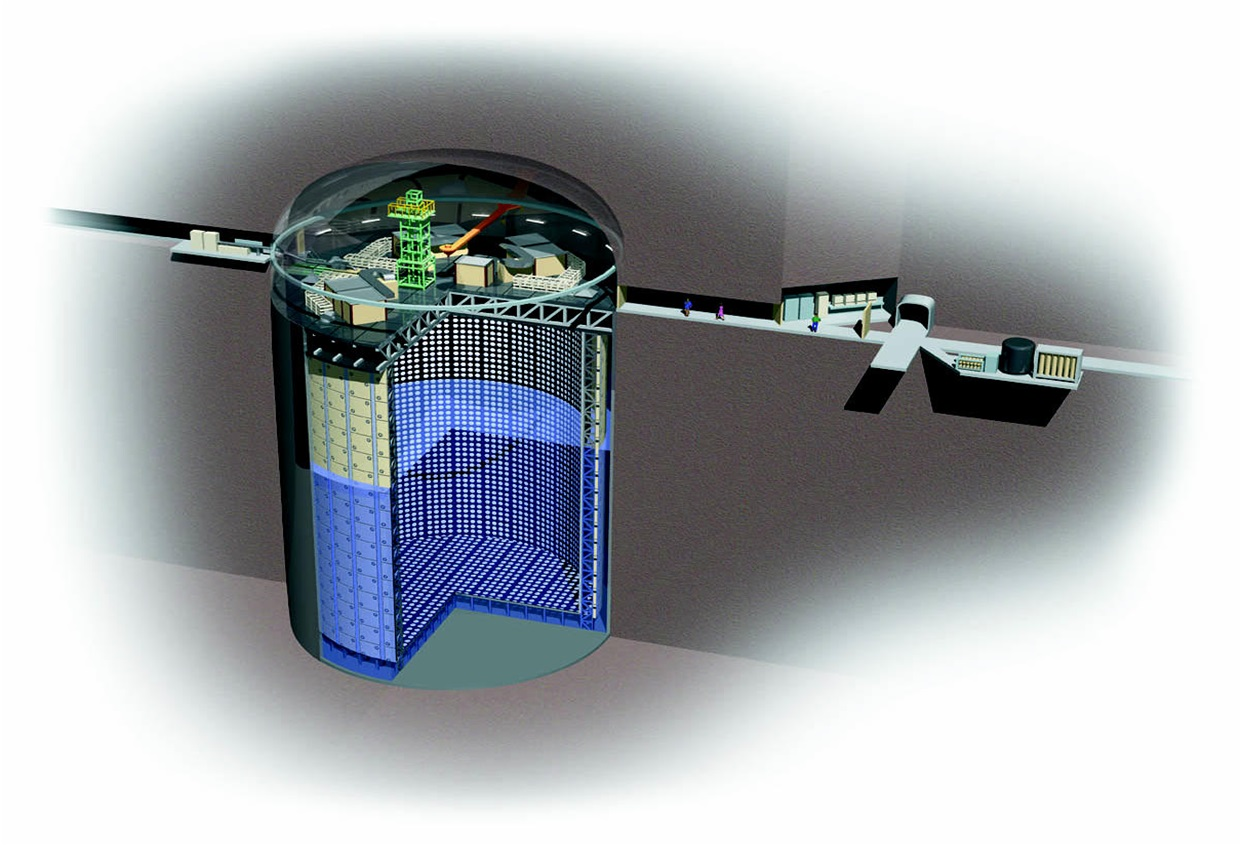
\includegraphics[width=\textwidth]{figures/SK3D.jpg}
\vspace{2mm}
  %\label{fig:sub1}
\end{subfigure}%
\begin{subfigure}{.5\textwidth}
  \centering
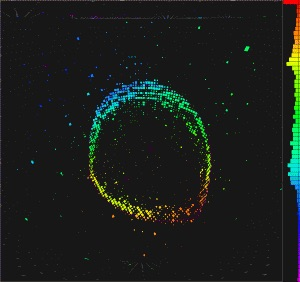
\includegraphics[width=0.7\textwidth]{figures/SuperKMuon-300x282.jpg}
\vspace{2mm}
  %\label{fig:sub2}
\end{subfigure}
\vspace{2mm}
\caption{Left) A schematic of the Super-K detector., Right) Event recorded in Super-K.}
\label{fig:SK}
\end{figure}
% http://t2k-experiment.org

\subsection{MACRO}
The Monopole, Astrophysics and Cosmic Ray Observatory (MACRO) detector (\FigRef{fig:macro}) was a combination of liquid scintillation counters, limited streamer tubes and nuclear track detectors which allowed it to search for signs of magnetic monopoles, as well as being able to operate as a neutrino detector and search for other phenomena. Data was taken between 1995 until 2000 and by measuring neutrino induced muons, the MACRO experiment managed to aid in the discovery of atmospheric neutrino oscillation~\cite{62MACRO}.

\begin{figure}[h!]
\centering
  \centering
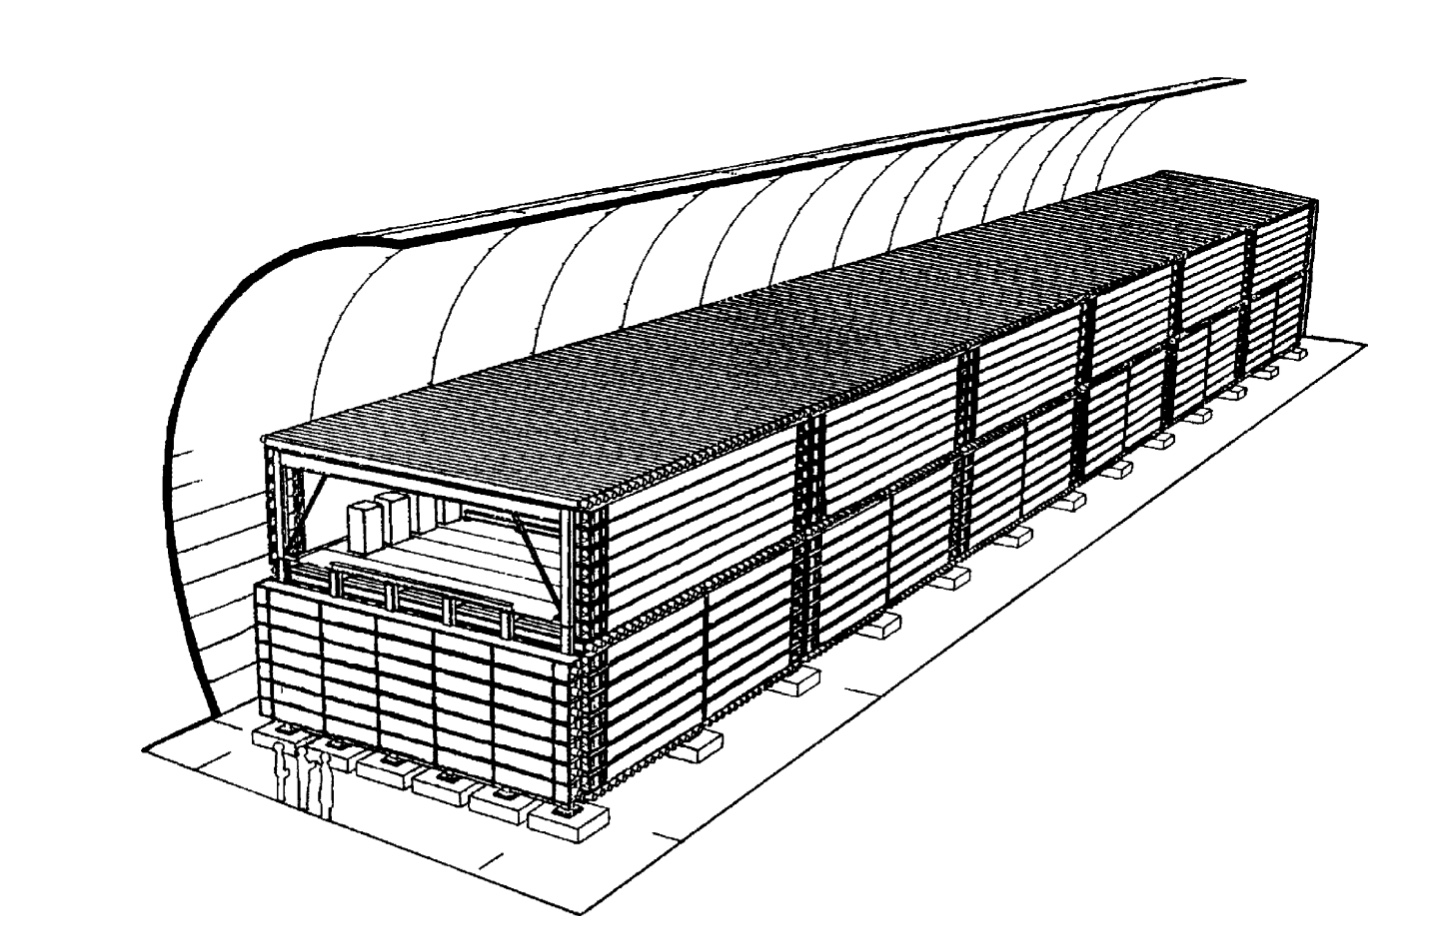
\includegraphics[width=0.49\textwidth]{figures/MACRO.jpeg}
\vspace{2mm}
\caption{Schematic of the MACRO detector~\cite{61MACRO}.}
\label{fig:macro}
\end{figure}

\pagebreak
\newpage
\section{Solar neutrino experiments}
The mechanism for neutrino generation in the sun was briefly discussed in subsection~\ref{subsection:Missing}.
Solar neutrinos are interesting for both allowing a unique way of probing the internal solar reactions  as well as providing a very long baseline for neutrino oscillations. Solar neutrino experiments are sensitive to $\theta_{12}$ and $\Delta m^2_{12}$.

% combined with energies of around $1 MeV/c$ allowing probing of mass differences in the range of $\Delta m^2 \approx 10^{-10} eV^2$ through neutrino oscillation, see equation~\ref{eq:twoPNeutrinoosc}. Based on current experimental values these experiments are sensitive for $\theta_{12}$ and $\Delta m_{12}^2 $

%Mention best values and different hierarchy?

\subsection{Super-KamiokaNDE}

%Super-KamiokaNDE, as described in subsection~\ref{subsection:Super-K} was sensitive enough to measure solar neutrinos with improved sensitivity. It was able to confirm the reduction of the solar electron neutrino flux $2:38 \pm 0:05(stat) ^{0:16}_{0:15} \times  10^6 cm^{-2} s^1$, and determine the solar neutrino parameters to be $\tan^2 \theta = 0.40$ and $\Delta m^2 \pm 6:03\times 10^5$~eV$^2$~\cite{64SuperK}.

Super-KamiokaNDE, as described in subsection~\ref{subsection:Super-K} was sensitive enough to measure solar neutrinos with improved sensitivity. It was able to confirm the reduction of the solar electron neutrino flux $(2.38 \pm 0.05(stat) ^{+0.16}_{-0.15}) \times 10^6$ $cm^{-2} s^1$, and determine the solar neutrino parameters to be $\tan^2 \theta = 0.40$ and $\Delta m^2 \pm 6.03\times 10^5$~eV$^2$~\cite{64SuperK}.

%Super-Kamiokande, as described above, could thanks to its design, also be used for solar neutrino studies and extended the neutrino oscillation analysis to lower mass difference values as well as performed solar interaction measurements~\cite{64SuperK}.

\subsection{SNO}
%It expanded on looking for a specific energy range for cosmic rays, from boron decay, to becoming a generic neutrino detector meaning that other atmospheric and cosmic neutrinos became background events for measuring solar neutrinos. 

The Sudbury Neutrino Observatory (SNO)~\cite{Fix6} was built to make a definite measurement of solar neutrinos following the measurements taken by the Homestake experiment~\cite{9Davis}. The observatory recorded data from 19999 to 2006. It utilized PMT (Photo Multiplier Tubes) to measure Cherenkov radiation produced by neutrino interactions in the detector's 1000 ton ultra-pure heavy water (D$_2$O) volume (\FigRef{fig:SNO}). The whole detector is placed 2 km underground to minimise background interactions. The larger depth of this experiment reduces the cosmic ray and atmospheric neutrino background seen by this detector and careful selection of materials used inside the detector reduced the threshold for solar neutrino interactions with respect to Super-K. The experiment has a unique ability to separate the reactions between electron neutrino charge current $\nu_e + d \rightarrow p + p + e^-$ (CC), neutral current interactions $\nu_x + d \rightarrow n + p + \nu_x$ (NC) with all flavours of neutrinos and with electron scattering $\nu_x + e^- \rightarrow \nu_x + e^-$ (ES). The neutrino flux observed through CC reactions could be compared to that of the ES  and NC to provide evidence for a neutrino flavour change regardless of the predictions of solar modes.

The experiment clearly showed a significant difference in flux between CC interactions, only available with electron neutrinos compared to expected and compared to the NC and ES interactions. The result can be seen in \FigRef{fig:SNO2}.

\begin{figure}[h!]
\centering
\begin{subfigure}{.5\textwidth}
  \centering
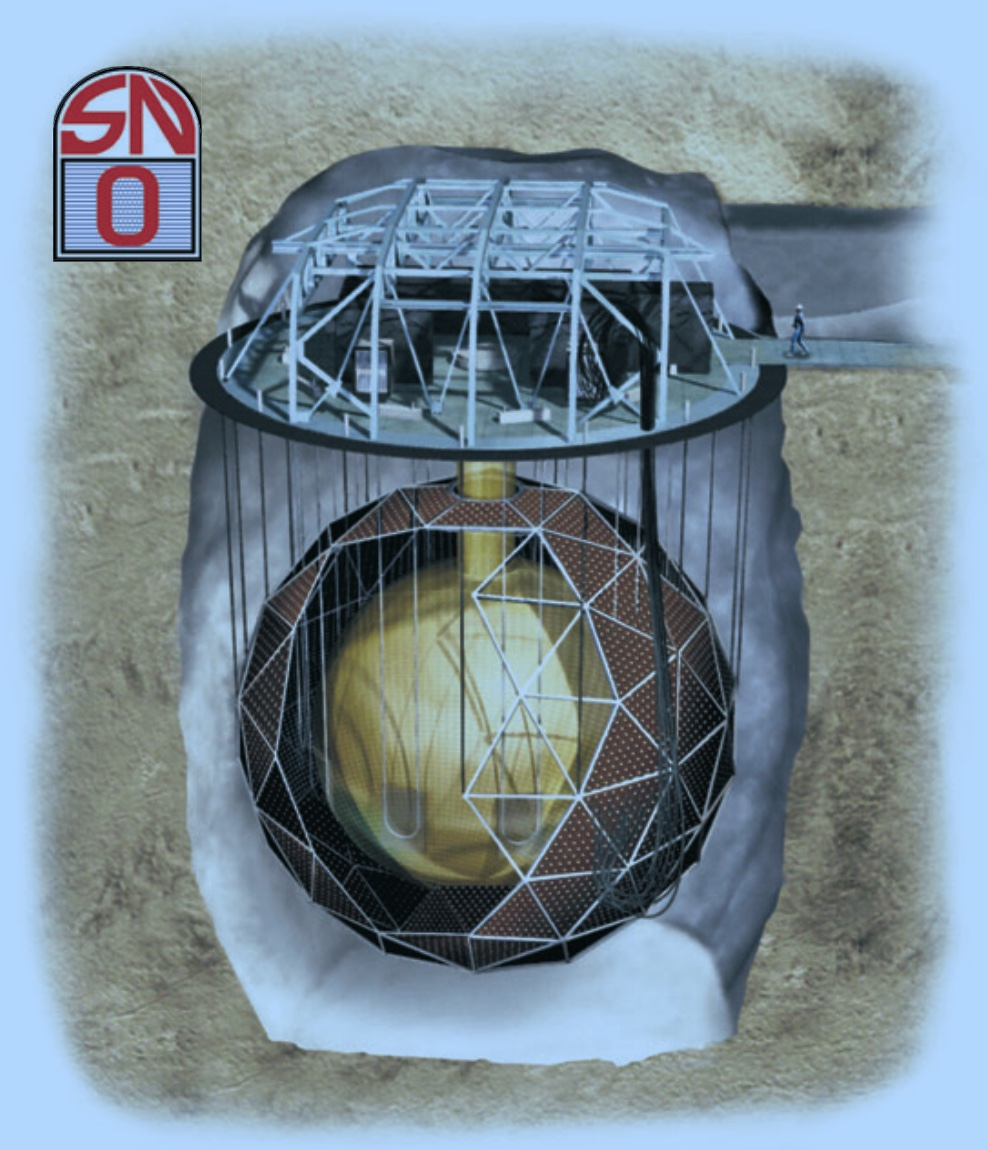
\includegraphics[width=0.7\textwidth]{figures/sno.jpeg}
\vspace{2mm}
  %\label{fig:sub1}
\end{subfigure}%
\begin{subfigure}{.5\textwidth}
  \centering
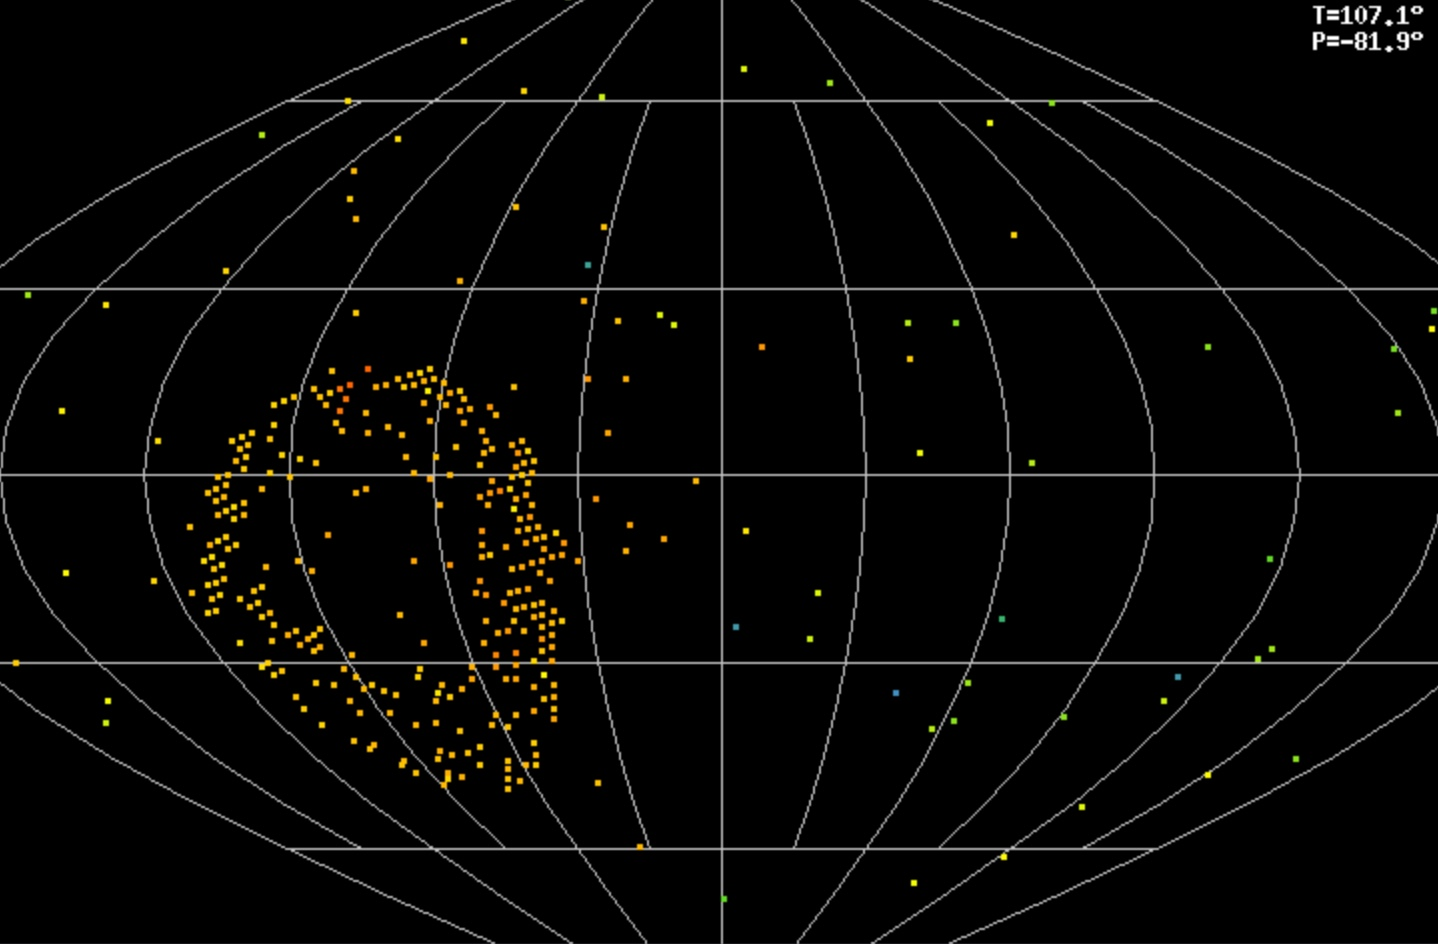
\includegraphics[width=\textwidth]{figures/SNOmuonEvent.jpeg}
\vspace{2mm}
  %\label{fig:sub2}
\end{subfigure}
\vspace{2mm}
\caption{Left) A schematic drawing of the SNO detector~\cite{Fix6}, Right) Cherenkov light recorded from a muon created by interaction of an atmospheric neutrino in the heavy water.}
\label{fig:SNO}
\end{figure}

\begin{figure}[h!]
\centering
  \centering
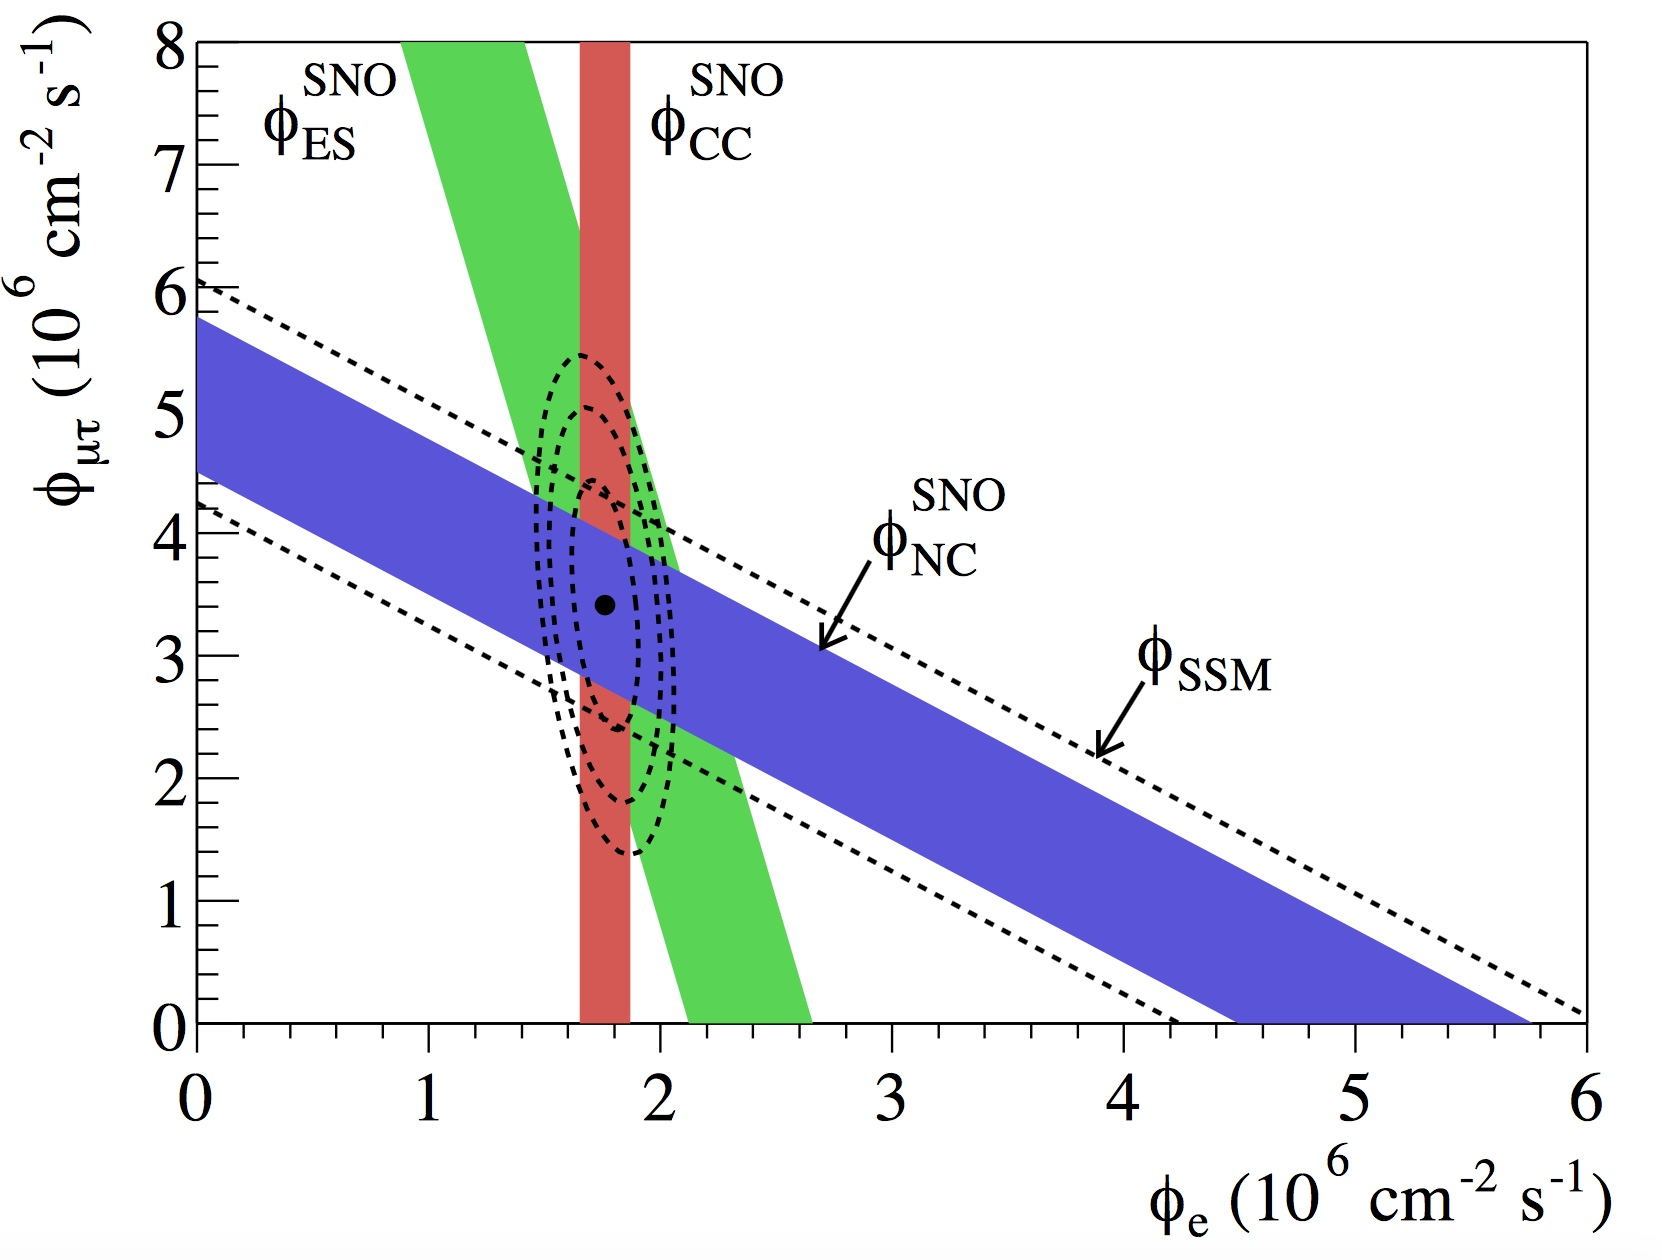
\includegraphics[width=0.49\textwidth]{figures/fixSNO.jpeg}
\vspace{2mm}
\caption{The flux of solar neutrinos of $\mu$ or $\tau$ flavour vs flux of electron neutrinos measured in SNO from the three reactions, CC in red, ES in green and NC in blue.The diagonal dashed lines show the prediction from the Standard Solar Model. The coloured bands intersect at the fit values for all fluxes indicating that they are consisted with neutrino flavour transformation with no distortion in the solar neutrino energy spectrum~\cite{98Ahmad}.}
\label{fig:SNO2}
\end{figure}

The experiment is currently replacing the heavy water with liquid scintillator and renaming itself as SNO+~\cite{42SNO+} to carry out a programme to search for double-beta decay.

\subsection{Borexino}
Borexino is a liquid scintillator detector with very small radioactive contamination background, making it more sensitive to low energy solar neutrinos than the SNO and Super-K water Cherenkov detectors, but it lacks the ability to determine the direction of the incoming neutrino, since scintillation light is isotropic. The low radioactive background is achieved by containing the detector within shielding material and utilizing ultra pure materials~\cite{63Borexino}. The scintillating light is then read out by PMTs uniformly distributed around the active volume seen in \FigRef{fig:borexino}.

The experiment started data taking in May 2007 and is still ongoing. It has the goal of making  very precise measurements of solar neutrino fluxes as well as setting limits on charge non conservation, limits on sterile neutrinos and measuring neutrinos emanating from the core of the earth (geoneutrinos).

\begin{figure}[h!]
\centering
  \centering
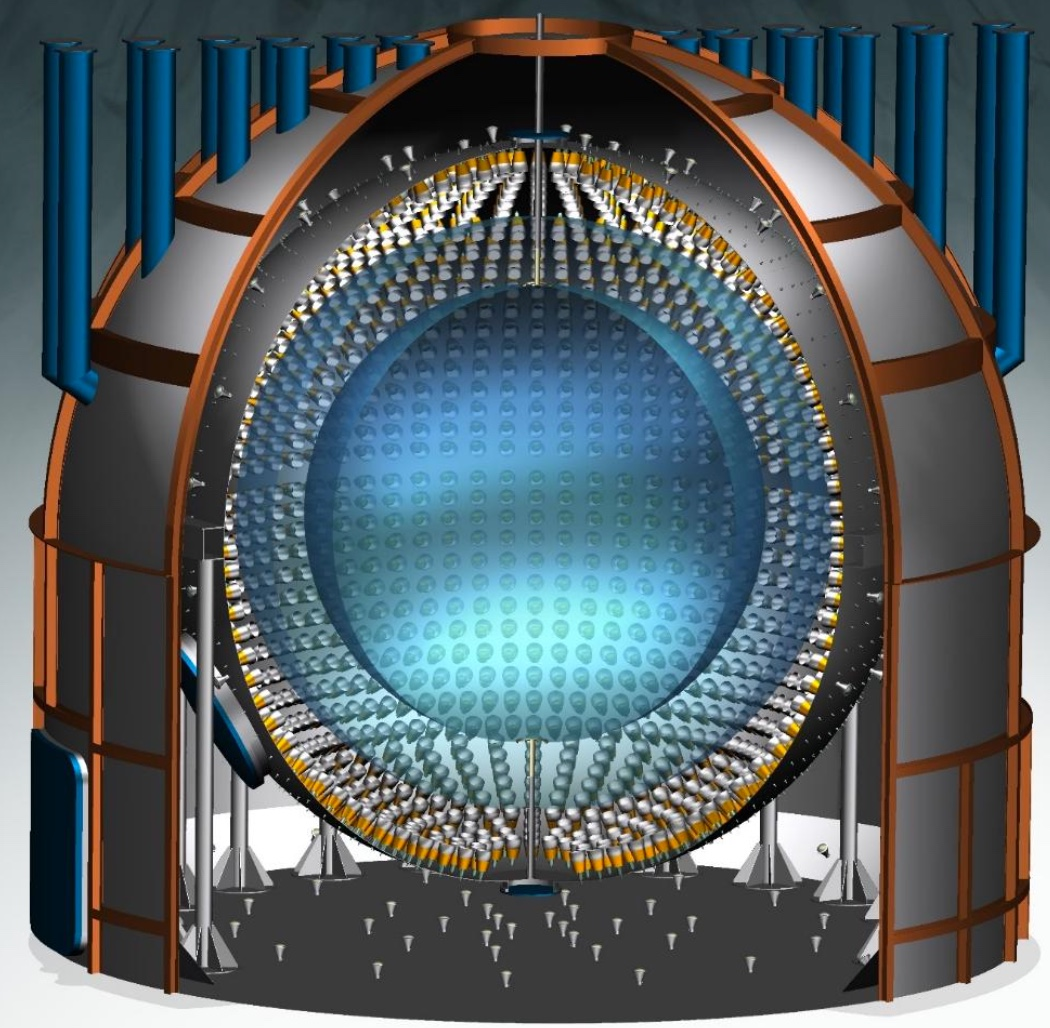
\includegraphics[width=0.49\textwidth]{figures/borexino.jpeg}
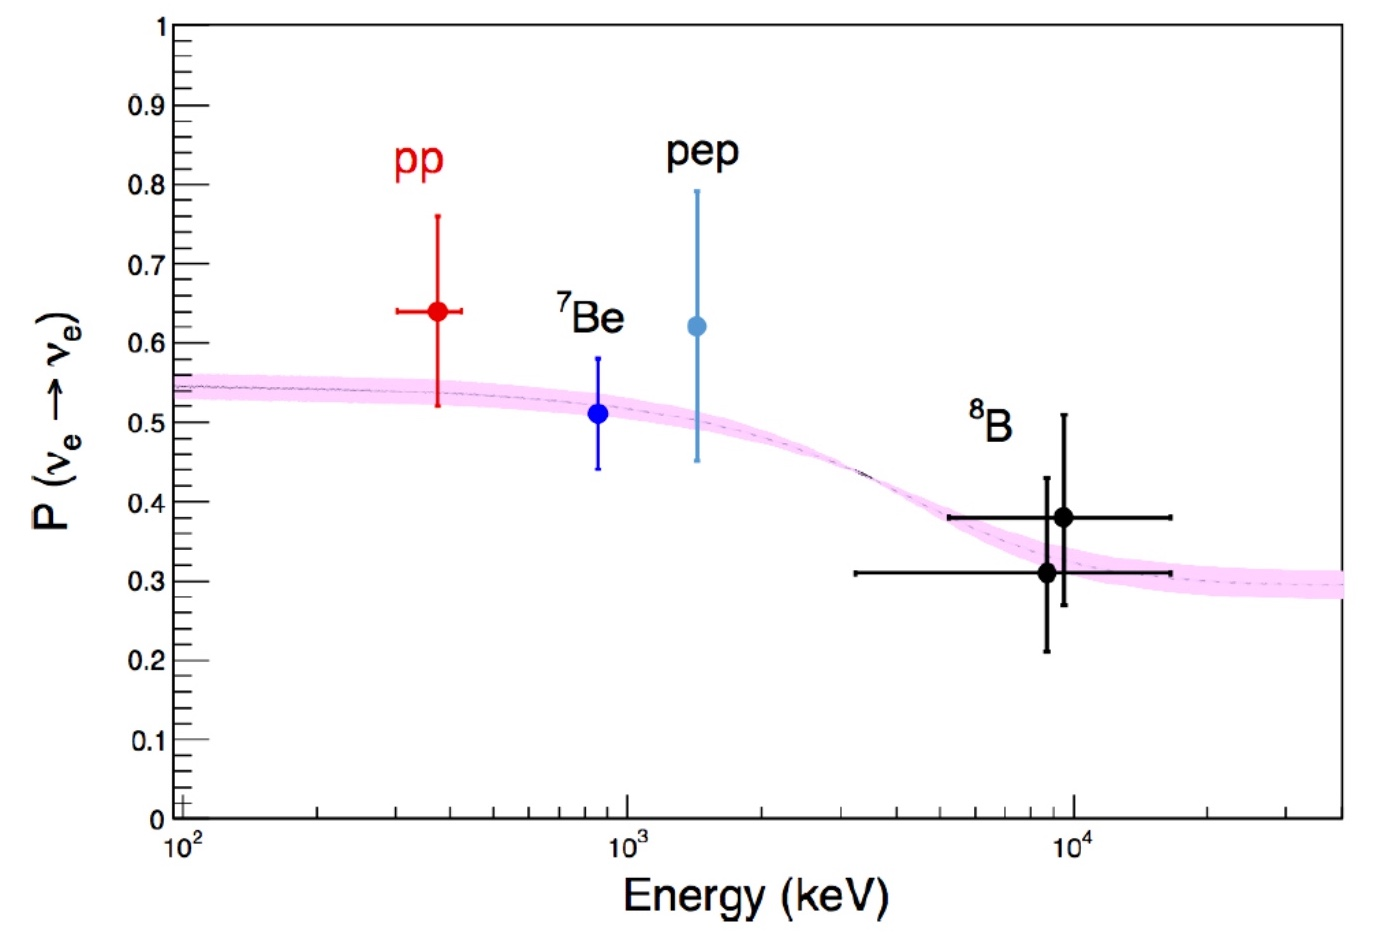
\includegraphics[width=0.49\textwidth]{figures/borexino3.jpeg}
\vspace{2mm}
\caption{(Left) Schematic of the Borexino experiment~\cite{63Borexino}. (Right) Electron neutrino survival probability as a function of neutrino energy measured by the Borexino experiment from different production channels predicted by the standard solar model~\cite{63Borexino}.}
\label{fig:borexino}
\end{figure}

\if{0}
\textbf{The most recent solar and terrestrial neutrino results stemmed from Borexino have further reinforced the ultra-low background achievements of this experiment, an exceptional breakthrough in the field of techniques for rare processes search. The 7Be, 8B, pep and the very recently measured pp components have all been detected (together with a tight upper limit on CNO), leading to the validation of the MSW-LMA oscillation paradigm in the entire energy regime of the solar neutrinos, strengthened also by the determination of the absence of day-night asymmetry in the 7Be flux. Very remarkably, Borexino performed this validation with its own data, without the need to resort to the results of other solar neutrino experiments.
Finally, the highly significant measurement of the terrestrial neutrinos not only complements the physics potentiality of the detector, but points towards a future new direction of research in the studies of the interior of the Earth.}
\fi

\pagebreak
\newpage
\section{Accelerator neutrino experiments}
Currently accelerator facilities can produce muon and electron neutrinos as well as antineutrinos from accelerated protons. Protons are accelerated in a particle accelerator and directed at a target where the protons interact with the target material, producing a large number of secondary pions (among other particles). Shaped magnetic fields, so-called focusing horns, are used to select out pions of the preferred charge (positive for a neutrino beam, negative for an antineutrino beam) in a specific momentum range and focus them into a collimated beam. The beam is directed into a long decay volume, where the pions decay into muons and (anti)neutrinos. At the end of the decay volume there is a large mass of material which absorbs all the particles except the neutrinos. This provides a nearly pure beam of muon-neutrinos (or muon-antineutrinos if negatively charged pions are selected). There is some inevitable contamination from antineutrinos in the neutrino beam or neutrinos in the antineutrino beam and from electron-neutrinos, mostly because the original pion beam also includes some kaons and muons, which can decay to produce electron-neutrinos. The main difference between accelerator-based neutrino experiments from the other types is that the beam composition is relatively well known. The energy range is higher than for reactor neutrinos. For oscillation experiments, the beam composition is generally measured using a near detector to determine any oscillation component at a far detector.

The advantages of accelerator neutrinos are that the energy range is well known and can be quite well tailored to the desired measurement and the flux is large compared to other methods. However the energy distribution will be quite wide because of the decay processes involved. It is also hard to produce a clean beam without background, for example, muon neutrinos without electron neutrinos. However, for oscillation experiments this can be desirable, see subsection \ref{subsec:nuFACT}. Based on current experimental values these experiments are sensitive for $\theta_{23}$ and $\Delta m_{23}^2 $.

\subsection{Historical experiments}
%The European Organization for Nuclear Research, (CERN) has had accelerator neutrino experiments and some based around magnetised volumes to provide change identification of particles. 

The European Organization for Nuclear Research (CERN) Dortmund Heidelberg Saclay Warsaw (CDHSW)~\cite{40CDHSW} experiment was designed to study neutrino interactions in iron using the CERN SPS neutrino beam line. The experiment consisted of two similar detectors at different distances from the interaction vertex 130 m and 885 m~\cite{40CDHSW}. The detectors were designed to combine the functions of a muon spectrometer and a hadron calorimeter. It consisted of 19 toroidal magnetised iron modules, with an average field of 1.65 T, separated from each other by wire drift chambers. The total detector mass was 1250 tons. A liquid hydrogen tank was placed in front of the experiment to study neutrino interactions in hydrogen. This is one of the first Magnetised Iron Neutrino Detectors (MIND).

The CHARM Collaboration (CERN-Hamburg-Amsterdam-Rome-Moscow Collaboration) proposed to study neutrino-nucleon and neutrino-electron interactions as well as muon polarisation. It took data from 1978 to 1991 and  was comprised of a fine-grained target calorimeter made up of 78 subunits each surrounded by a frame of magnetized iron for muon identification and spectrometry~\cite{68CHARM}.

The CCFR (University of Chicago, Columbia University, Fermilab, and the University of Rochester) detector installed at Fermilab consisted of an 18 m long 690 ton neutrino target calorimeter and followed by an iron toroid spectrometer. The calorimeter was made up of 168 iron plates, each 3m $\times$ 3m $\times$ 5.1cm, with liquid scintillation counters spaced between every two plates and drift chambers spaced every four plates. It provided among other things, precision measurements for neutrino-nucleon scattering~\cite{67CCFR}. The experiment was continued and became the NuTeV experiment which expanded results using the same detector and measured structure functions from deep inelastic scattering and electroweak parameters~\cite{99Yang, 100Zeller}. CCFR took data from 1979 to 1988, NuTeV started in 1996 and continued until 2003.

\subsection{NOMAD}
The Neutrino Oscillation Magnetic Detector (NOMAD)~\cite{NOMADexp}, also using the CERN SPS neutrino beam line, searched for $\nu_\mu \rightarrow \nu_\tau$ oscillation by detecting $\tau$ appearance~\cite{101Astierj} between 1995 and 1998. Its goals were to measure the momenta of charged particles and identify and measure electrons, photons and muons. By the detector design it was also possible to look for $\nu_\mu \rightarrow \nu_e$ oscillation~\cite{102Astier}. Compared to the modular design of CDHS, NOMAD had drift chambers and other sub-detectors contained inside a dipole magnet at 0.4 T (\FigRef{fig:NOMAD}).


%\textbf{RESULTS?}
\begin{figure}[h!]
\centering
  \centering
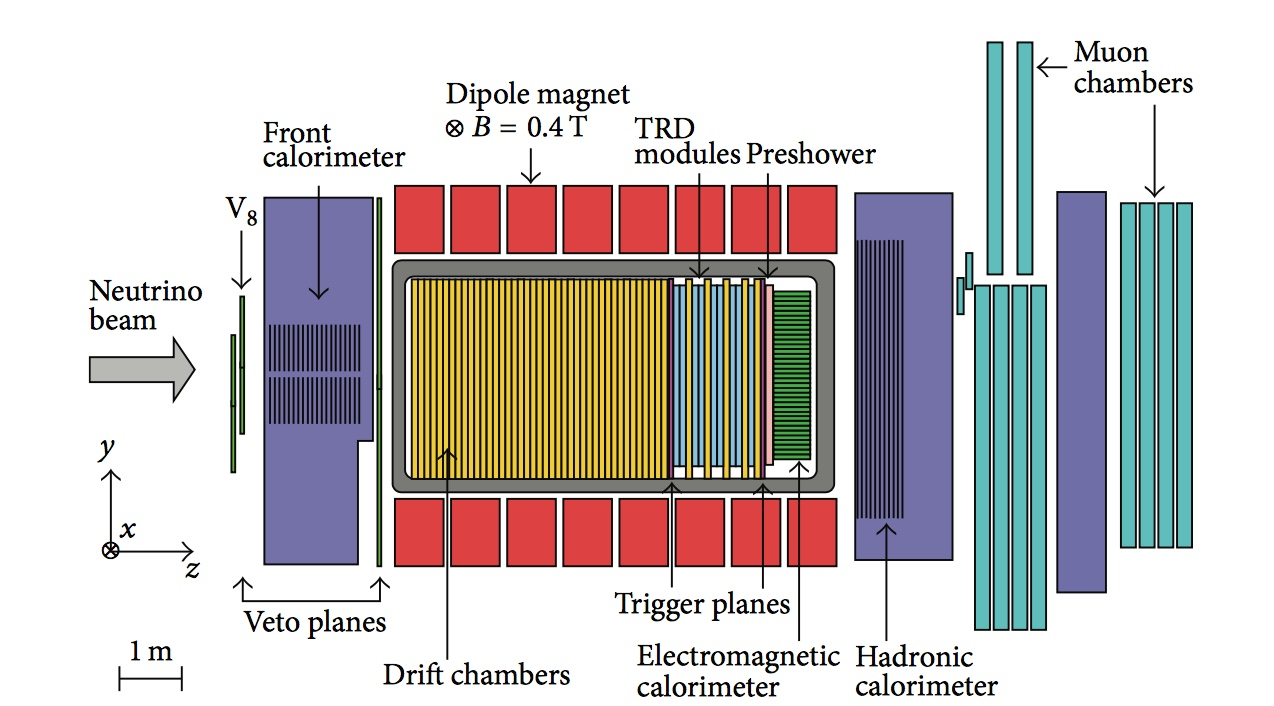
\includegraphics[width=0.7\textwidth]{figures/NOMAD2.jpeg}
\vspace{2mm}
\caption{A sideview of the NOMAD detector~\cite{69NOMAD}.}
\label{fig:NOMAD}
\end{figure}

\subsection{K2K}
After the success of Super-Kamiokande, the High Energy Accelerator Research Organization (KEK) to Kamiokande (K2K) experiment ~\cite{22K2K} was created with the main difference of using a well understood muon neutrino beam pointing at the Super-Kamiokande detector at a distance of 250 km. It was the first long-baseline neutrino oscillation measurement to observe the disappearance of muon neutrinos into tau neutrinos and found results of mass difference and mixing angle obtained that were consistent with Super-Kamiokande.

K2K, the set up seen in~\FigRef{fig:K2K}, ran from 1999 to 2004 and used a neutrino beam with a wide spectrum peaked at 1 GeV based on a 12 GeV proton synchrotron beam interacting with an aluminium target and focused through two horns and allowed to decay in a 200 m long decay pipe. This created a 98\% pure muon neutrino beam with around 1\% contamination of anti muon neutrinos and around 1\% electron and anti-electron neutrinos. Understanding the beam composition is required for looking at $\nu_\mu$ disappearance. To do this a 1-kiloton water Cherenkov near detector,  a scaled-down version of Super-Kamiokande, was used to measure the neutrino spectrum which is then extrapolated using Monte Carlo simulated data to predict the neutrino spectrum at Super-Kamiokande.

\begin{figure}[h!]
\centering
  \centering
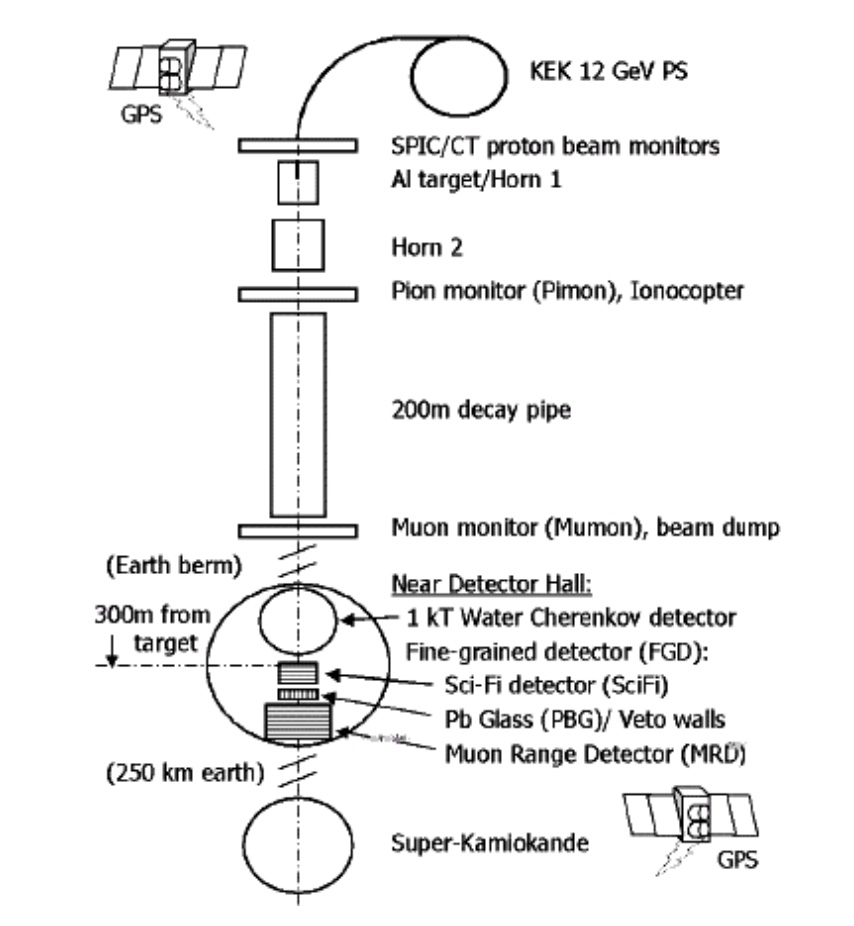
\includegraphics[width=0.7\textwidth]{figures/KEK.jpeg}
\vspace{2mm}
\caption{A schematic view of the K2K experiment~\cite{70K2K}.}
\label{fig:K2K}
\end{figure}

\subsection{MINOS, NOvA and MINERvA}
%\url{http://www-numi.fnal.gov/Minos/minospub.txt}

The Main Injector Neutrino Oscillation Search (MINOS)~\cite{MINOS} is a muon neutrino disappearance experiment, consisting of two magnetised spectrometers, one near (1 km from the target) and one far detector (735 km from the target), and using the NuMI~\cite{19NuMI} beam at Fermilab. The experiment took data from 2005 to 2012.

The two detectors have been designed to be as similar as possible to minimize any systematic errors in comparing the observed neutrino spectra in the two detectors. They are both constructed of planes with two magnetised steel plates with layers of scintillator in between, to measure the charge and momentum of charged particles and to allow their discrimination. The far detector is composed of 486 octagonal plates with a diameter of 8 meters and total length of 30 meters providing a total mass of 5400 tons. The near detector contains only 282 planes, slightly squashed octagonal planes at 3.8 meters $\times$ 4.8 meters. MINOS showed results consistent with Super-Kamiokande and the K2K experiments such as observation of $\nu_\mu$ disappearance, measurements of the mixing angle and the mass squared difference.

After MINOS the next step using the NuMI~\cite{19NuMI} beam is the NOvA~\cite{18nova} experiment, which is an electron neutrino appearance experiment and hopes to be able to determine the mass hierarchy of neutrinos with initial results published in~\cite{103NOVA}.

The MINERvA (Main INjector ExpeRiment $\nu$-A) experiment \cite{39minerva} also uses the NuMI~\cite{19NuMI} beam to study neutrino-nucleus scattering to improve models of neutrino-nucleus scattering to reduce systematic uncertainties in results from oscillation experiments.

%MiniBooNE\cite{41MiniBooNE} continued on what was started by MINOS but had the principle aim on improving neutrino mass measurements.

\subsection{T2K}
%\textbf{Correct after Pauls comments and add data.}

%\textbf{Here or in chap 3?}

After the success of K2K, the T2K experiment~\cite{21T2K} started data taking in 2010. This is a long-baseline neutrino oscillation experiment with a more powerful beam from the Japanese Proton Accelerator Research Complex (J-PARC) facility at Tokai to Super-Kamiokande, at a distance of 295 km, with a near detector inside an underground hall in Tokai, at a distance 280 m from the target, see~\FigRef{fig:T2K}.

The neutrino beam comes from an initial 30 GeV/c proton beam which impinges onto a graphite target embedded inside a magnetic horn. After the target the secondary beam is passed through two magnetic horns and focused into a decay volume before passing the beam dump. From here there is $\approx180$ meters of soil until hitting the near detector hall. This means that the near detector is traversed by neutrinos with an expected flux as seen in~\FigRef{fig:ND280Flux}, and by muons from neutrino interaction in the soil upstream of the near detector. The magnetic horn can be tuned to provide a neutrino spectrum, forward mode, or anti-neutrino spectrum, reverse mode, by charge selecting the primary particles from the proton interaction.

%This is all completely out of context, since you have not introduced INGRID. I suggest that you add two more paragraphs in the T2K section in chapter 2 in which you explain the near detectors of T2K, including the ND280 off-axis detector and the INGRID on-axis detector. If you add this in section 2.4.5 then this paragraph will make sense.
%Interactive Neutrino GRID (INGRID)~\cite{85INGRID}.

\begin{figure}[h!]
\centering
  \centering
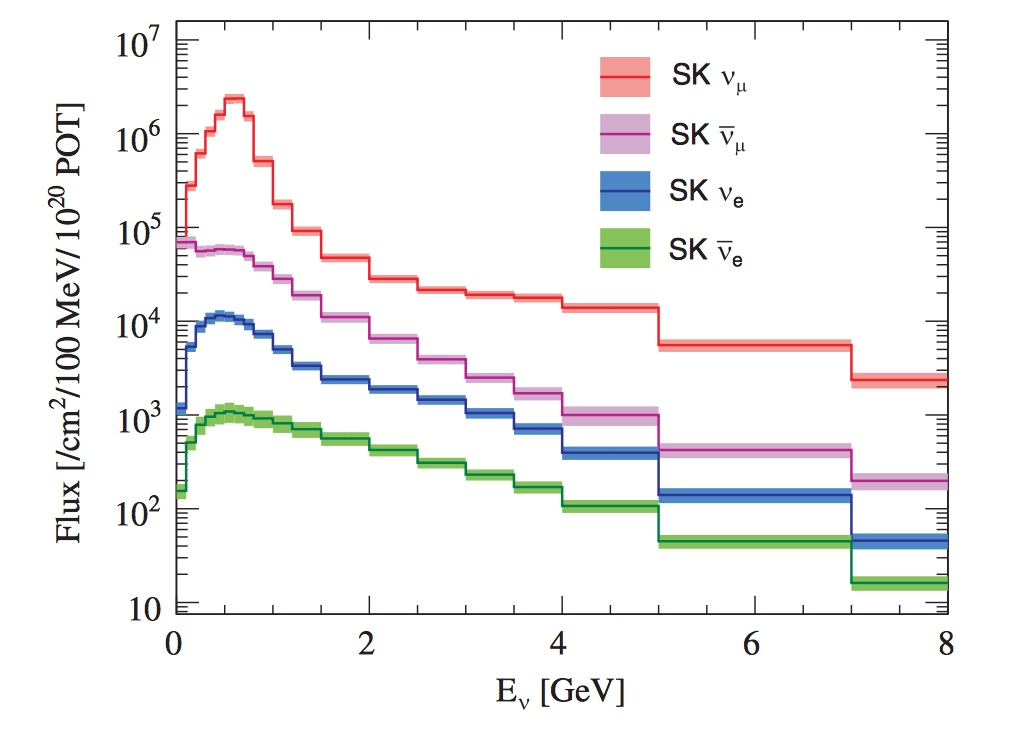
\includegraphics[width=\textwidth]{figures/ND280Flux.jpeg}
\vspace{2mm}
\caption{Simulated unoscillated expected neutrino fluxes for various flavours at the Super-K position for a forward horn current focussed beam, with expected systematic errors plotted as bands before applying the near detector data~\cite{21T2K}.}
%\caption{Simulated unoscillated expected neutrino fluxes for various flavours with expected systematic before applying near detector data plotted as bands. at Super-K~\cite{21T2K}.}
\label{fig:ND280Flux}
\end{figure}

\begin{figure}[h!]
\centering
  \centering
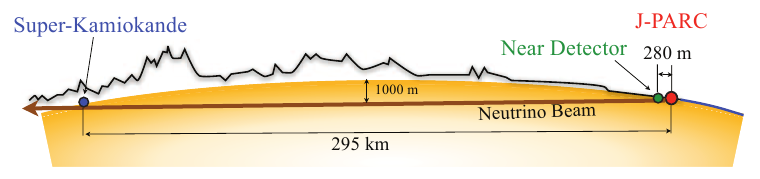
\includegraphics[width=\textwidth]{figures/T2KBeam.png}
\vspace{2mm}
\caption{A schematic view of the T2K experiment, including the near detector site ND280 and Super-K~\cite{21T2K}.}
\label{fig:T2K}
\end{figure}

The near detector hall contains two main experiments, an on-axis experiment INGRID~\cite{129INGRID} (\FigRef{fig:INGRIDdet}) and the off-axis ($2.5^\circ$) ND280 detector~\cite{130Assylbekov} (\FigRef{fig:ND280det}) both used to reduce model uncertainty and systematic uncertainty in the Super-Kamiokande analysis. %\textbf{More details?}

The experiment wants to improve our understanding of the neutrino oscillation parameters. T2K was able to successfully observe the appearance of muon to electron neutrino oscillations and find evidence that the third mixing angle $\theta_{13}$ is not zero. 

The combined analysis shows the sensitivity of the experiment to the CP violating phase $\delta_{CP}$ (figure 2.16), the measurements of neutrino mixing parameters obtained by T2K (\FigRef{fig:T2K23}) and the effect of the measurement of $\theta_{13}$ as a function of the value of $\delta_{CP}$ (\FigRef{fig:T2K12}). This is still an ongoing experiment with ongoing analyses.

%The combined analysis showing the affect of the $\theta_{13}$ value on $\delta_{CP}$ is seen in . 

%Here you should include the latest results from T2K, the \theta_{13}$ measurements with the electron neutrino appearance analysis and the sensitivity to CP violation. You should discuss these results and motivate the results you show in figures 2.16 and 2.17, including full references.

\begin{figure}[h!]
\centering
  \centering
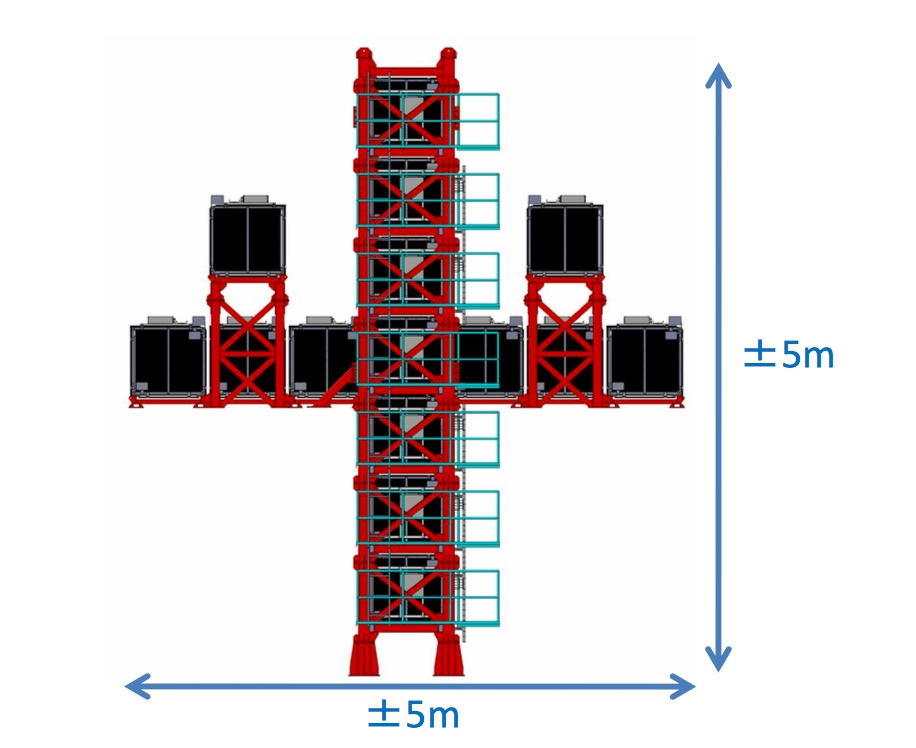
\includegraphics[width=0.7\textwidth]{figures/ingridPlot.jpeg}
\vspace{2mm}
\caption{The INGRID on-axis near detector. the center of the cross, with two overlapping modules, corresponds to the designed neutrino beam center~\cite{129INGRID}.}
\label{fig:INGRIDdet}
\end{figure}

\begin{figure}[h!]
\centering
  \centering
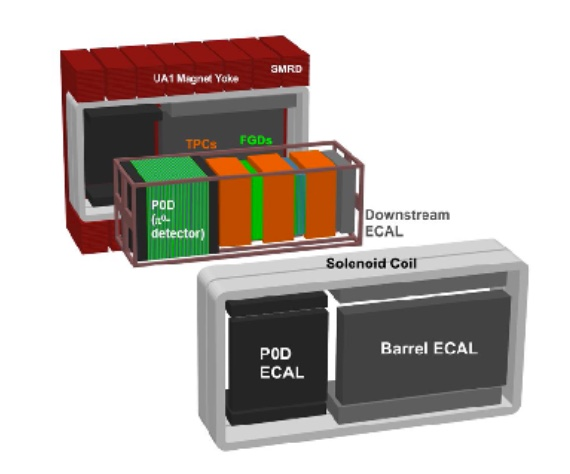
\includegraphics[width=0.7\textwidth]{figures/ND280det.jpeg}
\vspace{2mm}
\caption{An exploded view of the ND280 detector~\cite{130Assylbekov}.}
\label{fig:ND280det}
\end{figure}

\begin{figure}[h!]
\centering
  \centering
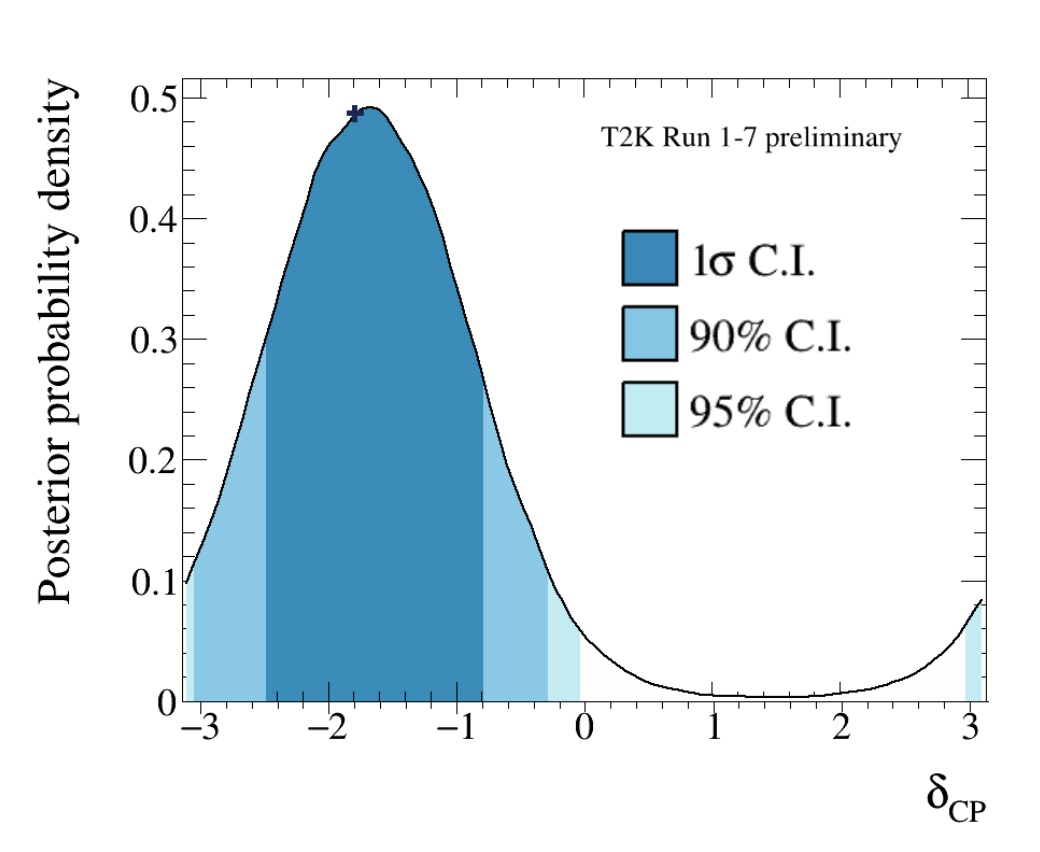
\includegraphics[width=0.7\textwidth]{figures/t2k1.jpeg}
\vspace{2mm}
\caption{Posterior probability density on $\delta_{CP}$, where the cross represent the best-fit~\cite{T2Kfigures}.}
\label{fig:T2KCP}
\end{figure}

\begin{figure}[h!]
\centering
  \centering
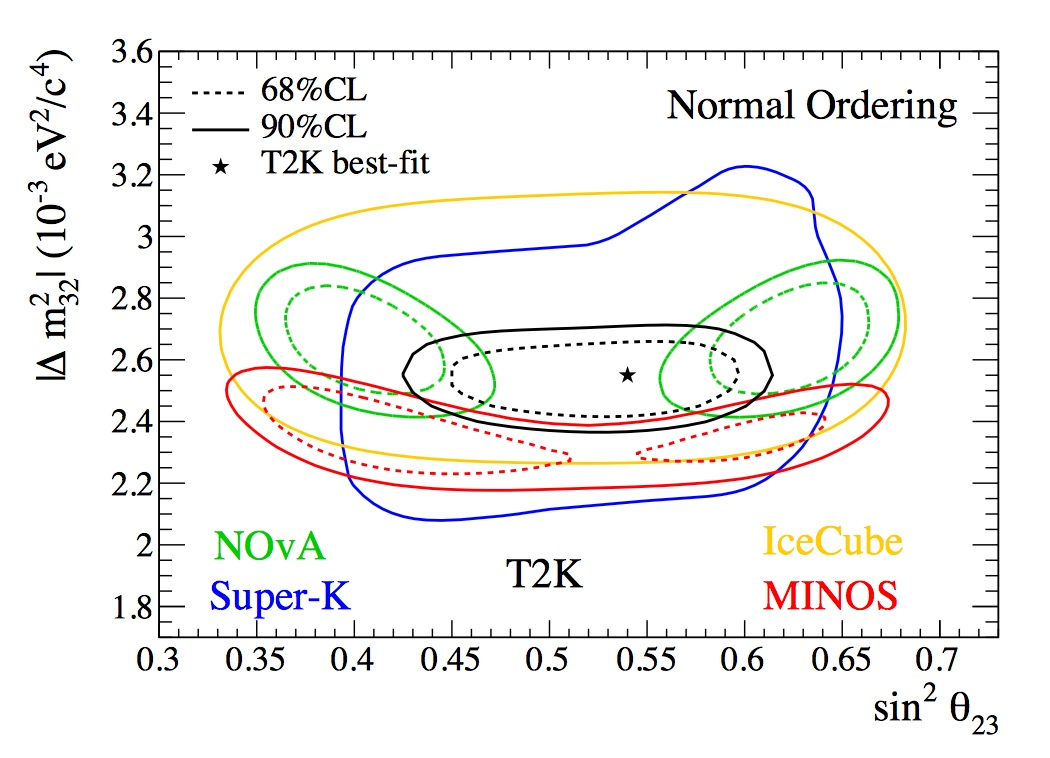
\includegraphics[width=0.7\textwidth]{figures/t2k2.jpeg}
\vspace{2mm}
\caption{The 90\% and 68\% confidence levels in the $\sin^2 \theta_{23}, \Delta m^2_{32}$ space from T2K compared to other experiments, assuming normal ordering of neutrino masses~\cite{T2Kfigures}.}
\label{fig:T2K23}
\end{figure}

\begin{figure}[h!]
\centering
  \centering
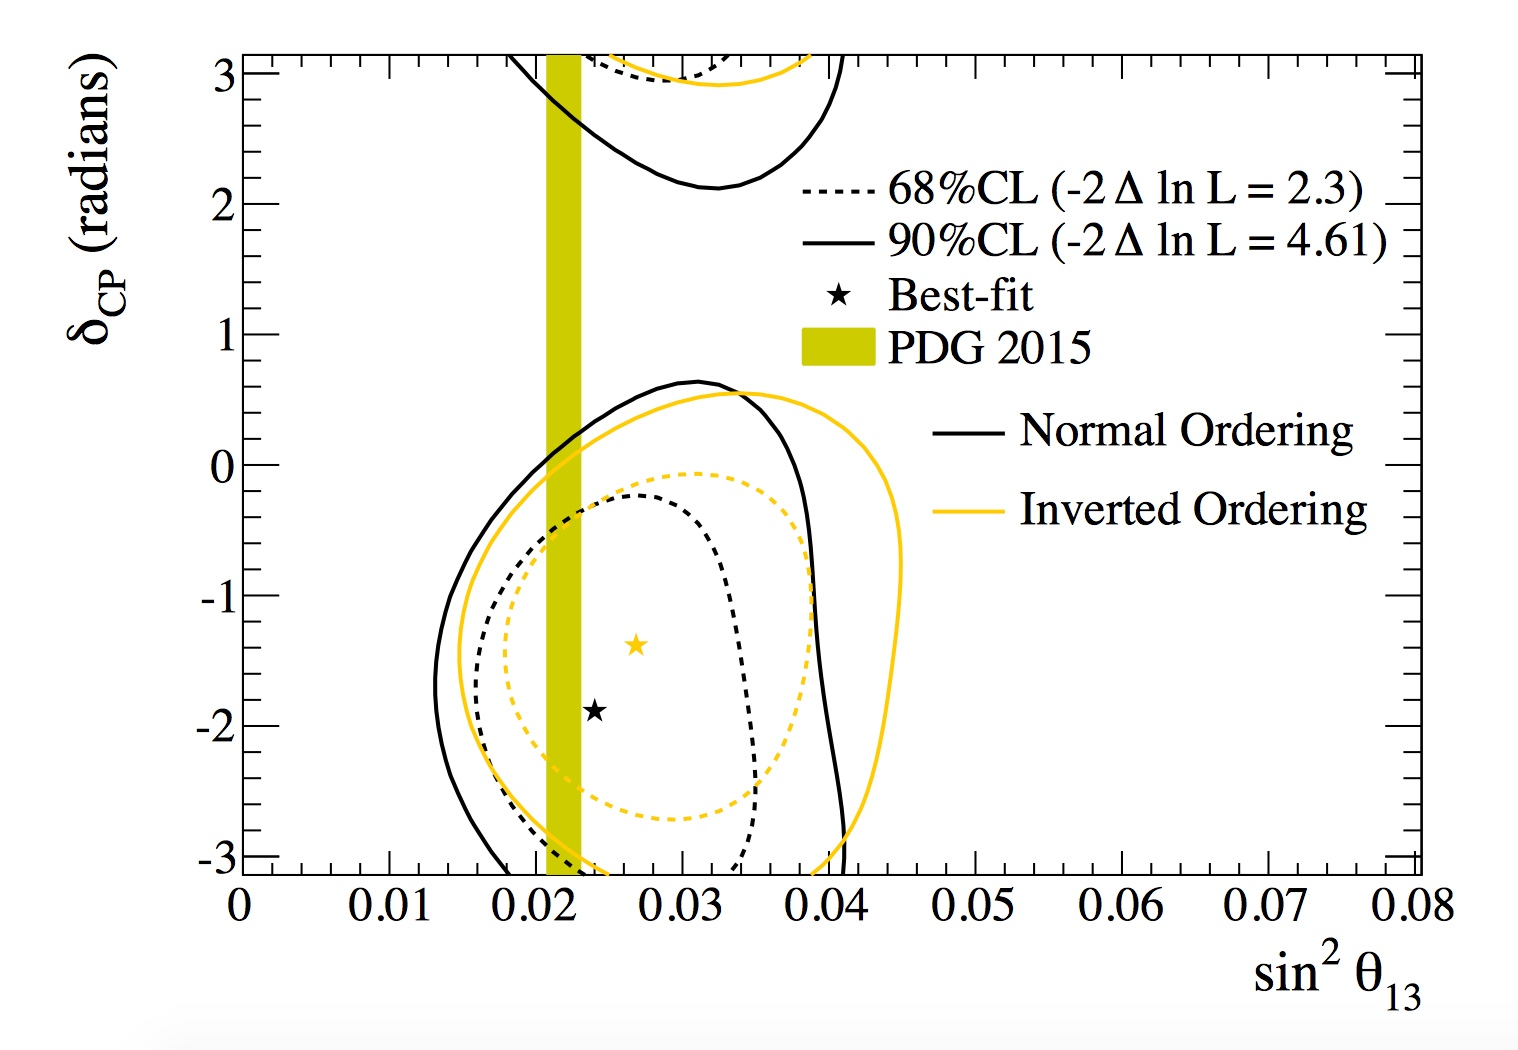
\includegraphics[width=0.7\textwidth]{figures/t2kfix.jpeg}
\vspace{2mm}
\caption{The 68\% and 90\% confidence regions in the $\delta_{CP} - \sin^2 \theta_{13}$ plane as the dashed and continuous lines for the normal (black) and inverted (red) mass ordering. The best-fit point is shown by a star for each mass ordering hypothesis. The 68\% confidence region of $\sin^2 \theta_{13}$ from reactor experiments is shown by the yellow vertical band~\cite{108Abe}.}
\label{fig:T2K12}
\end{figure}

One of the main sources of systematic error for T2K is caused by the difference of the target material and acceptance between the ND280 near detector (hydrocarbon) and the far detector water Cherenkov detector~\cite{T2Kpaper} motivating further studies and upgrades to ND280.

\pagebreak
\newpage
\FloatBarrier
\section{Reactor neutrino experiments}
Nuclear reactors are very intense sources of low energy neutrinos. Through beta-decay channels electron antineutrinos are produced with well known energy spectra and low background. Compared to other neutrino sources the energy range is limited to below 9 $MeV/c$, (see~\FigRef{fig:reactor}) as well as a sharp cut off at 1.8 $MeV/c$ required for inverse beta decay to occur. The low energy range means that oscillation experiments must be performed with a short baseline since equation~\ref{eq:twoPNeutrinoosc} provides the same probability by decreasing both the momentum and baseline.

Beta-decay is also relatively easy to detect as the positron deposits its kinetic energy in the scintillator and annihilates with an electron and generates two photons. These two photons and the deposited energy causes a so-called prompt signal a few nanoseconds after the neutrino event. The ejected neutron thermalises and produces a delayed signal about 20 ms later, which is a very clear signature of a neutrino event. 

The low energy range also means that experiments based on reactor neutrinos can only search for $\bar{\nu_e}$ disappearance since the produced neutrinos do not have enough energy to produce muons or taus and any neutral current interaction will be very difficult to distinguish from background. Based on the current values, neutrino reactor experiments are well suited to determine $\theta_{12}$ and $\Delta m_{12}^2 $ as well as  $\theta_{13}$ and $\Delta m_{13}^2$.

\begin{figure}[h!]
\centering
  \centering
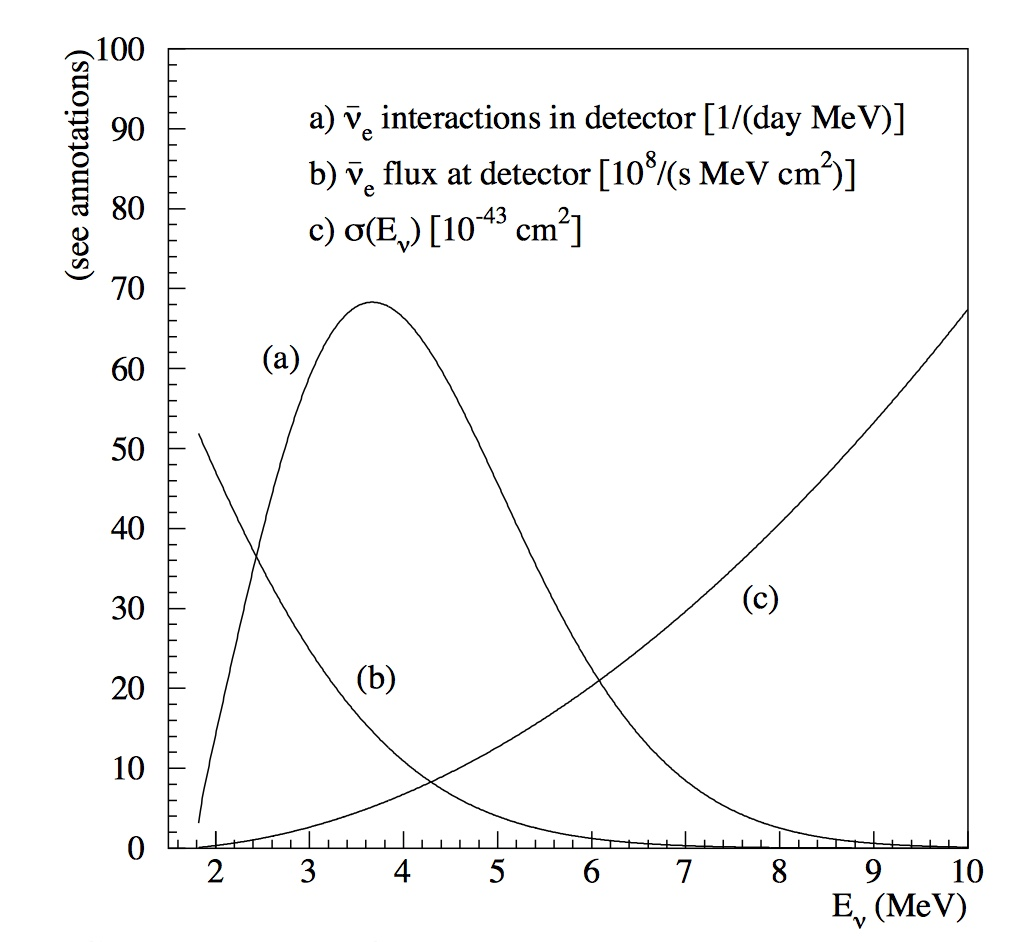
\includegraphics[width=0.7\textwidth]{figures/reactor.jpeg}
\vspace{2mm}
\caption{Energy spectrum of $\bar{\nu_e}$, the inverse beta decay cross section and interaction spectrum of detected inverse beta decay events~\cite{65Reactor}.}
\label{fig:reactor}
\end{figure}

\subsection{KamLAND}
After the completion of the KamiokaNDE experimental run, the site was used to install the Kamioka Liquid Scintillator Antineutrino Detector (KamLAND) in 2002. KamLAND, seen in \FigRef{fig:KamLAND}, looks specifically for neutrino oscillations by looking at  electron antineutrinos emitted from distant reactors~\cite{46KamLAND} by using a 1 kton liquid scintillator volume encased in oil. %If the neutrinos interact with the volume by inverse beta-decay, it will produce positrons which will annihilate and produce two distinct photon signals, known as prompt signal.

The majority of the neutrino events are from 26 reactors within the distance range of 138-214 km providing a good baseline to see oscillations by measuring distortions of the expected neutrino energy spectrum. The spectrum and results can be seen in \FigRef{fig:KamLAND2}. 

KamLAND showed that electron antineutrinos oscillate in the same way as the electron neutrinos from the sun and the results produce the same mixing angle and mass squared difference. These results confirm the oscillation parameters between electron and muon neutrinos in a completely independent way. The experiment also set a constraint on the value of $\theta_{13}$ before this was conclusively measured by Daya Bay~\cite{107Gando}. %Combining this result with other experiments measuring  $\theta_{12}$ and $\theta{23}$ as non-zero opened up the possibility of measuring $\delta_{CP}$ as discussed and showed in equation~\ref{eq:alignThreeFlavour}.

\begin{figure}[h!]
  \centering
  \begin{minipage}[b]{0.49\textwidth}
    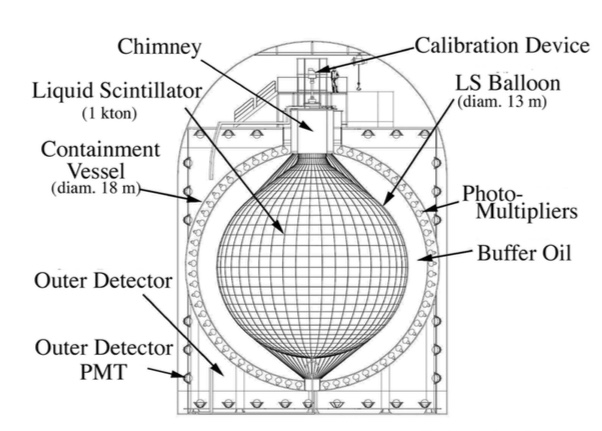
\includegraphics[width=\textwidth]{figures/KamLAND.jpeg}
    \vspace{2mm}
    \caption{Schematic diagram of the KamLAND detector~\cite{46KamLAND}.}
    \label{fig:KamLAND}
  \end{minipage}
  \hfill
  \begin{minipage}[b]{0.49\textwidth}
    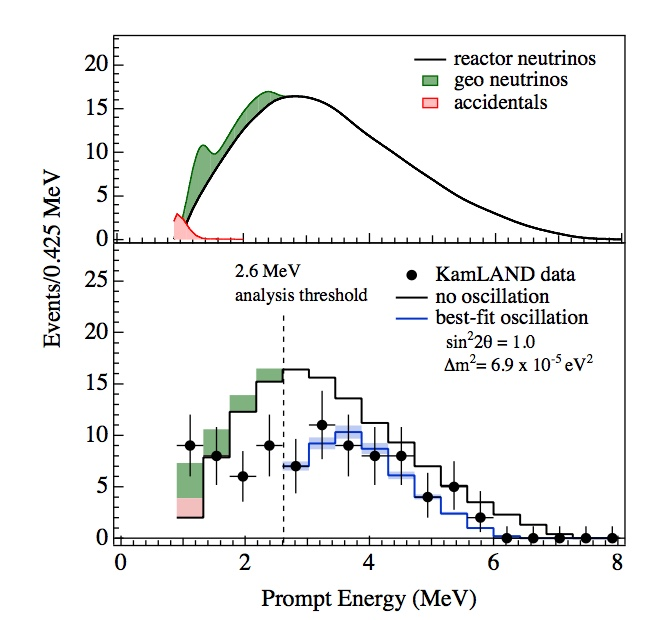
\includegraphics[width=\textwidth]{figures/KamLAND2.jpeg}
       \vspace{2mm}
    \caption{Top panel: Expected reactor $\bar{\nu_e}$ energy spectrum. Lower panel: Energy spectrum of the observed events along with the the no-oscillation spectrum and best-fit spectrum~\cite{46KamLAND}. }
     \label{fig:KamLAND2}
  \end{minipage}
\end{figure}

\subsection{Daya Bay}
%\textbf{Correct after Pauls comments and add data.}

The Daya Bay experiment's main result and goal was to make a conclusive measurement of $\theta_{13}$. The experiment measured  $\theta_{13}$ to be non-zero with more than 5$\sigma$ significance~\cite{122An} in 2012.

The Daya Bay Reactor Neutrino Experiment is a facility consisting of eight identical gadolinium-doped  liquid scintillator detectors placed in underground experimental halls at three locations around the Daya Bay area in China, which detect antineutrinos from six different nuclear reactor cores of thermal energy 2.9 GW$_{th}$ (figures 2.22 and 2.23). The flux-weighted baselines from the reactors to the three locations are 470 m and 576 m (two at a near location) and 1648 m, at a far location.

This layout allows for maximum sensitivity and the ability to reduce systematic uncertainties due to uncertainties in reactor power levels. It also allows for cross-calibration of the detectors since they are all identical. Each detector is a segmented gadolinium-doped liquid scintillator detector using PMTs to read out photons produced through inverse beta-decay and annihilation. %The experiment has been taking data since 2011.
The experiment has been taking data since 2011, and was the first experiment to measure a non-zero value for the neutrino mixing angle $\theta_{13}$ with more than 5$\sigma$ significance \cite{122An}. The search for electron-antineutrino disappearance is dependent on the $\theta_{13}$ mixing angle. The probability for antineutrino disappearance is given by
\begin{equation}
P(\bar{\nu}_e \rightarrow \bar{\nu}_e)\approx 1 - \sin^2(2\theta_{13}) \sin^2\left(\frac{1.27 L(m) \Delta m^2_{31} (eV^2) }{E_{\bar{\nu}} (MeV)} \right) . 
\end{equation}
The reduction in the reactor antineutrino flux is used to determine the value of $\theta_{13}$. Further measurements have improved on the original results, and now $\theta_{13}$ is the most accurately measured mixing angle of the neutrino sector \cite{123An, 124An}:
$\sin^2 2\theta_{13} = 0.0841 \pm 0.0027(stat) \pm 0.0019(syst)$ and the
effective neutrino mass-squared difference is $\Delta m^2_{ee} = (2.50 \pm 0.06(stat) \pm 0.06(syst)) \times 10^{-3}$~eV$^2$.

\begin{figure}[h!]
  \centering
  \begin{minipage}[b]{0.49\textwidth}
    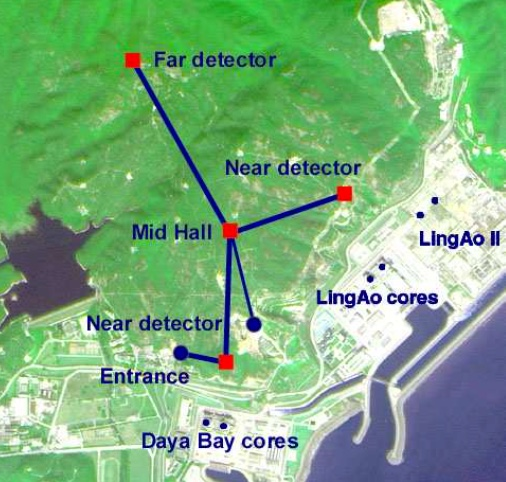
\includegraphics[width=\textwidth]{figures/DayaBay.jpeg}
    \vspace{2mm}
    \caption{Layout of the Daya Bay experiment~\cite{122An}.}
    \label{fig:DB}
  \end{minipage}
  \hfill
  \begin{minipage}[b]{0.49\textwidth}
    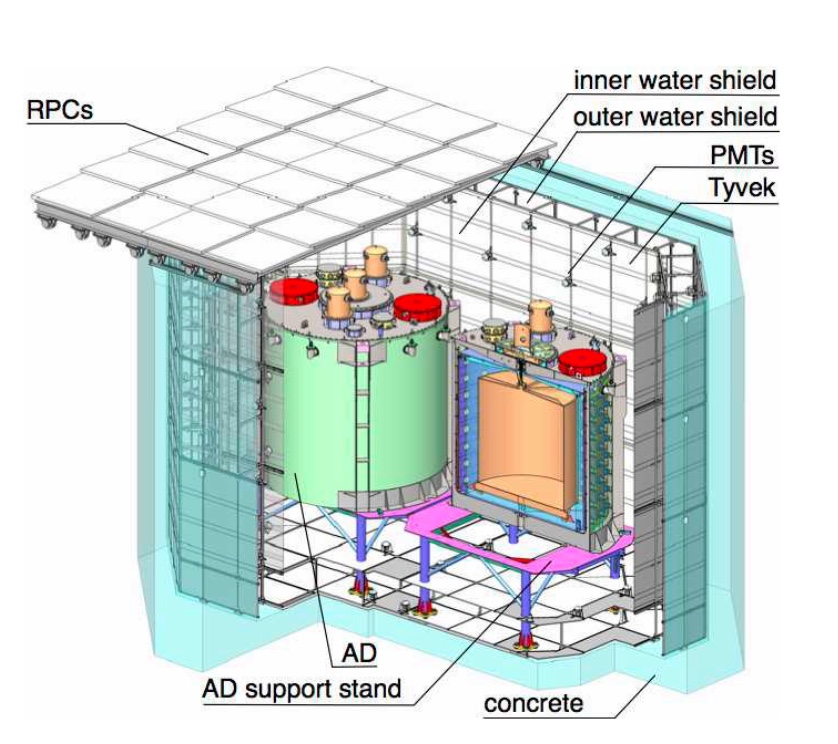
\includegraphics[width=\textwidth]{figures/db2.jpeg}
       \vspace{2mm}
    \caption{Near site layout of the Daya Bay detector with surrounding structure~\cite{122An}.}
     \label{fig:db2}
  \end{minipage}
\end{figure}

\begin{figure}[h!]
  \centering
  \begin{minipage}[b]{0.49\textwidth}
    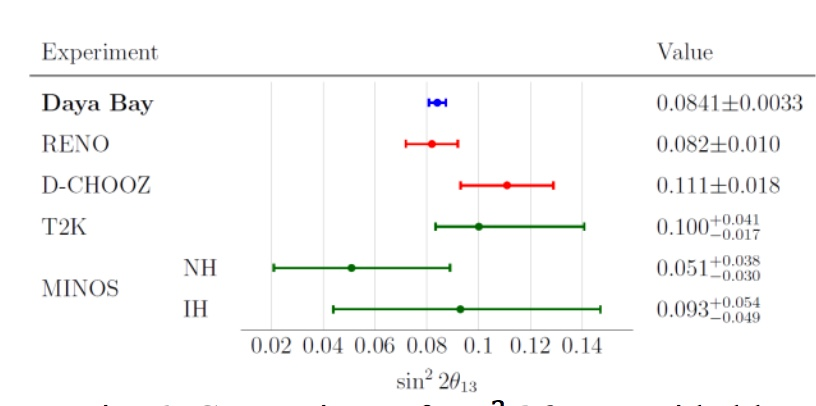
\includegraphics[width=\textwidth]{figures/db3.jpeg}
    \vspace{2mm}
    \caption{Comparison of $\sin^2 2\theta_{13}$ measurements from various experiments, taken from~\cite{122An}.}
    \label{fig:db3}
  \end{minipage}
  \hfill
  \begin{minipage}[b]{0.49\textwidth}
    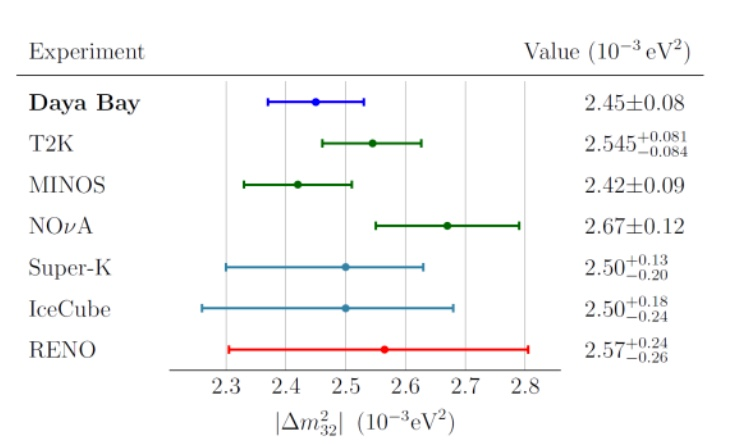
\includegraphics[width=\textwidth]{figures/db4.jpeg}
       \vspace{2mm}
    \caption{Comparison of $|\Delta m^2_{32}|$ measurements from various experiments, taken from~\cite{122An}.}
     \label{fig:db4}
  \end{minipage}
\end{figure}

\subsection{RENO}
The Reactor Experiment for Neutrino Oscillation (RENO), started taking data in 2011 and used two identical detectors placed at a near and far site. The detectors are liquid scintillator detectors with 16.5 tons of gadolinium-doped scintillator. It measures neutrinos generated by six nuclear reactors each spread out perpendicular from a base line setting the detectors at 294 m and 1383 m from the center of the base line, see~\FigRef{fig:reno1}. RENO measured $|\Delta m^2_{32}| = (2.61 \pm 0.16 \pm 0.09) \times 10^{-3} eV^2$ and $\sin^2(2\theta_{13}) = 0.086 \pm 0.006 \pm 0.005$ using the data in~\FigRef{fig:reno2} and confirmed the results from the Daya Bay experiment~\cite{125Ahn, 126RENO}.

\begin{figure}[h!]
  \centering
  \begin{minipage}[b]{0.49\textwidth}
    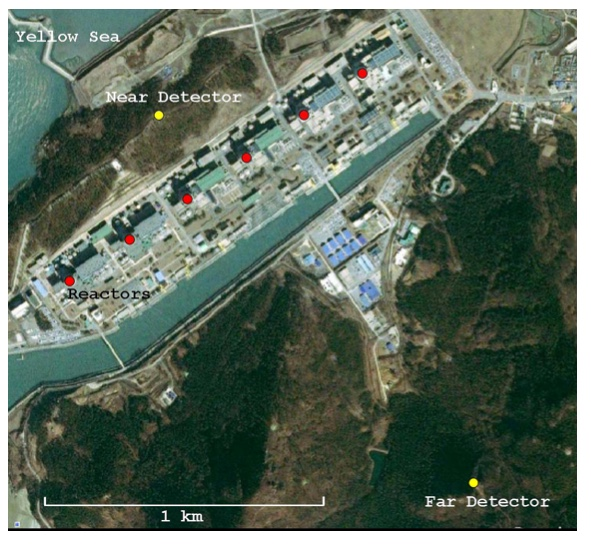
\includegraphics[width=\textwidth]{figures/reno1.jpeg}
    \vspace{2mm}
    \caption{Layout of the RENO detectors, yellow and reactors in red. The six reactors are equally spaced in a 1280 m span~\cite{125Ahn, 126RENO}.}
    \label{fig:reno1}
  \end{minipage}
  \hfill
  \begin{minipage}[b]{0.49\textwidth}
    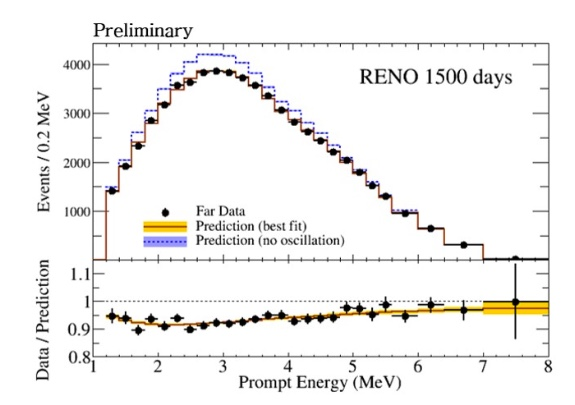
\includegraphics[width=\textwidth]{figures/reno2.jpeg}
       \vspace{2mm}
    \caption{Top panel: Measured energy spectrum with data on best fit and no oscillation models. Lower panel: Ratio of data over no-oscillation prediction~\cite{125Ahn, 126RENO}.}
     \label{fig:reno2}
  \end{minipage}
\end{figure}

\subsection{Double Chooz}
The Double Chooz experiment~\cite{127Abe, 128Abe} began in 2004 and used anti-neutrinos produced in two nuclear cores from a nuclear power station to measure the neutrino mixing angle $\theta_{13}$ as well as showing that these detectors can be used to ensure non-proliferation~\cite{45DoubleChooz, 66ReactorNP}. The experiment included two liquid scintillator detectors at a distance of 280 m and 1050 m, both consisting of photo-multiplier tubes (PMT) inside a scintillating volume shielded from cosmic radiation (\FigRef{fig:dc}). The disappearance spectrum from Double Chooz is seen in~\FigRef{fig:dc2}~\cite{72Double}.

\begin{figure}[h!]
  \centering
  \begin{minipage}[b]{0.49\textwidth}
    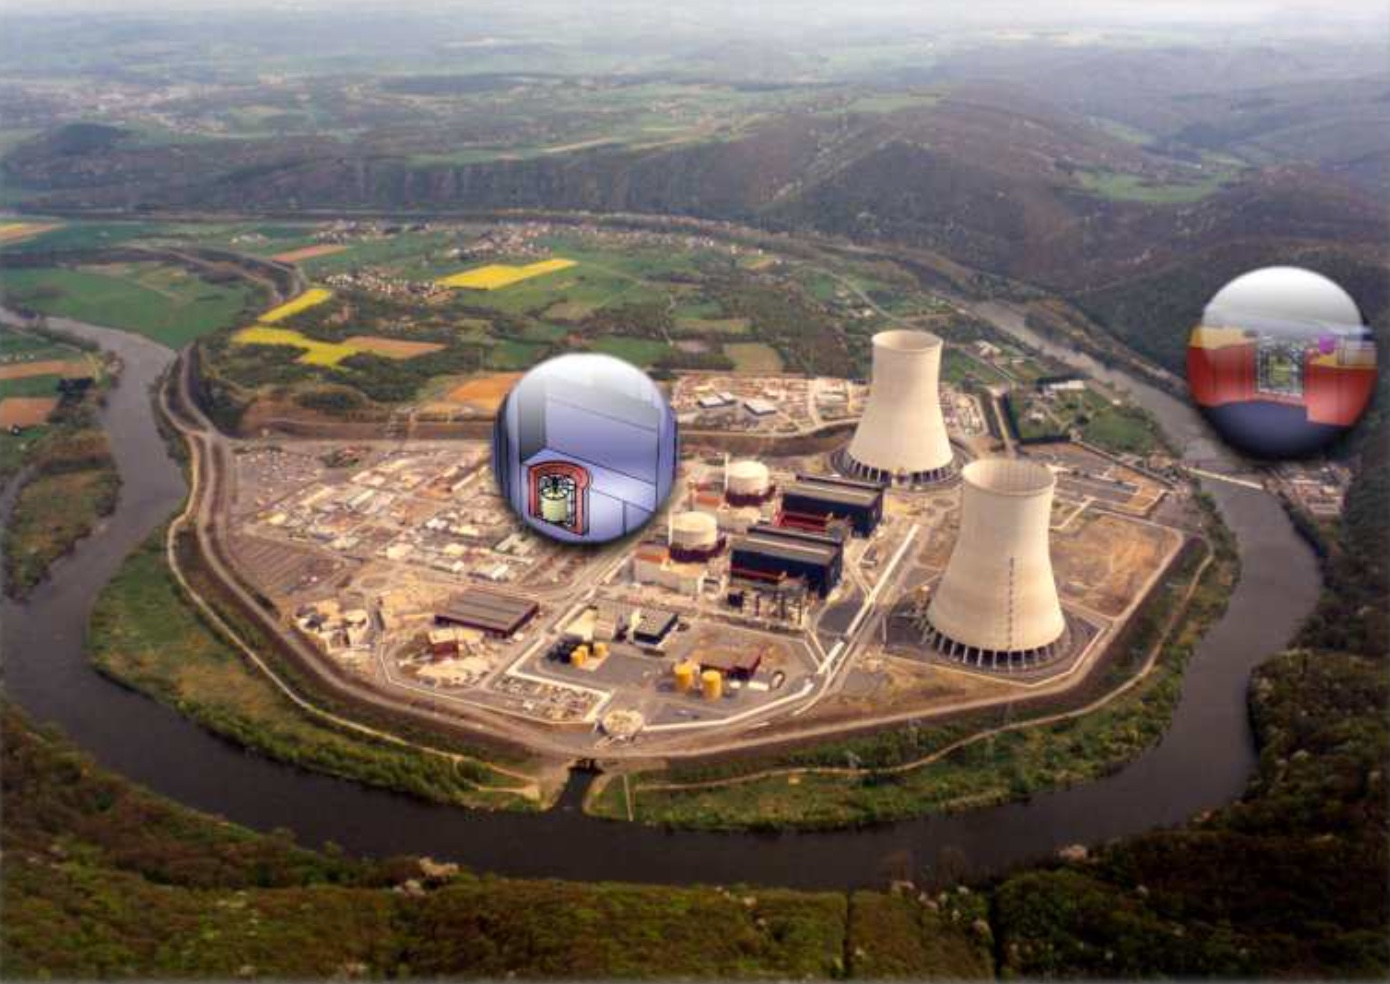
\includegraphics[width=\textwidth]{figures/doubleChooz.jpeg}
    \vspace{2mm}
    \caption{Overview of the Double Chooz experimental site~\cite{45DoubleChooz}.}
    \label{fig:dc}
  \end{minipage}
  \hfill
  \begin{minipage}[b]{0.49\textwidth}
    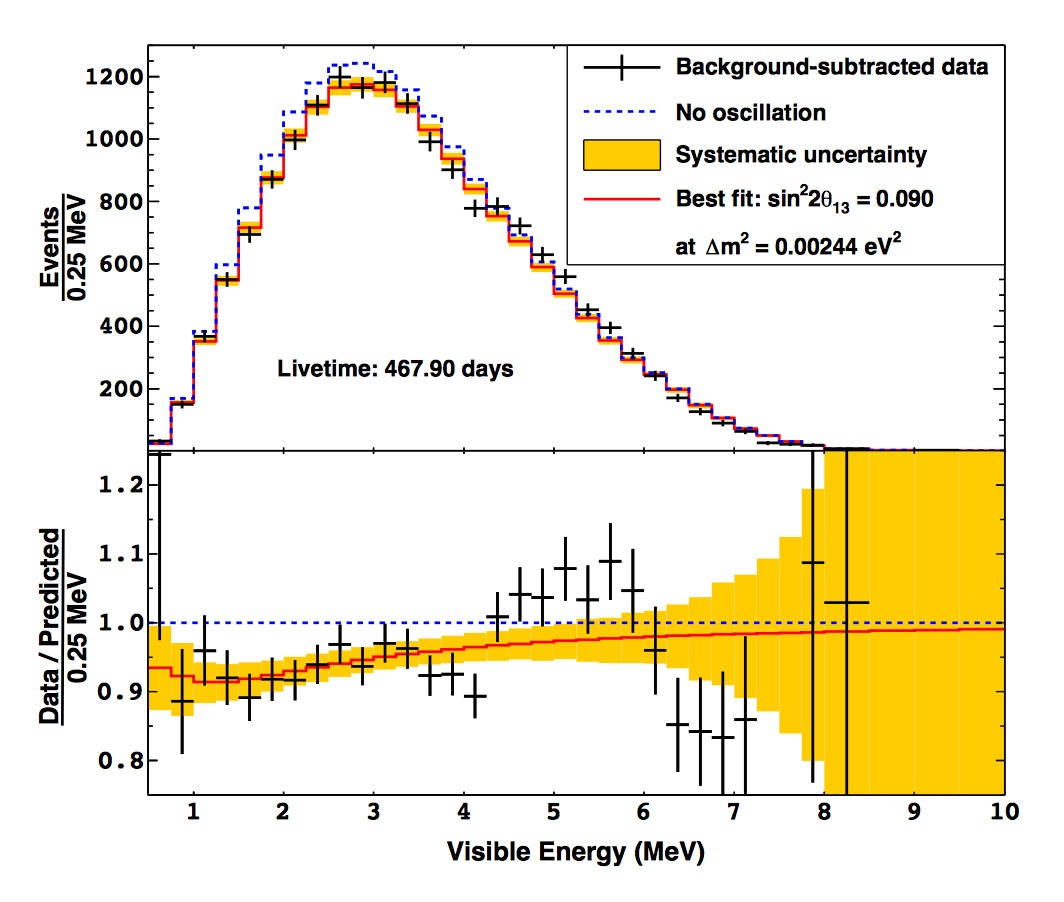
\includegraphics[width=\textwidth]{figures/doubleChooz2.jpeg}
       \vspace{2mm}
    \caption{Top panel: Measured energy spectrum with data on best fit and no oscillation models. Lower panel: Ratio of data over no-oscillation prediction~\cite{72Double}.}
     \label{fig:dc2}
  \end{minipage}
\end{figure}

\subsection{JUNO}

The Jiangmen Underground Neutrino Observatory (JUNO)~\cite{75Juno} is a 20 kton liquid scintillator detector currently under construction and aiming to start data taking in 2020, seen in both \FigRef{fig:juno1} and \FigRef{fig:juno2}. It has as one of its primary aims to determine the mass hierarchy, i.e. the sign of the mass splitting between the $m_2$ and $m_3$ mass eigenstates by using reactor neutrinos and inverse beta-decay with an improved energy resolution compared to previous experiments~\cite{75Juno}. It will use the Daya Bay set of reactors as a source of antineutrinos and results from the Daya Bay experiment to reduce systematic errors from the reactor.

\begin{figure}[h!]
  \centering
  \begin{minipage}[b]{0.49\textwidth}
    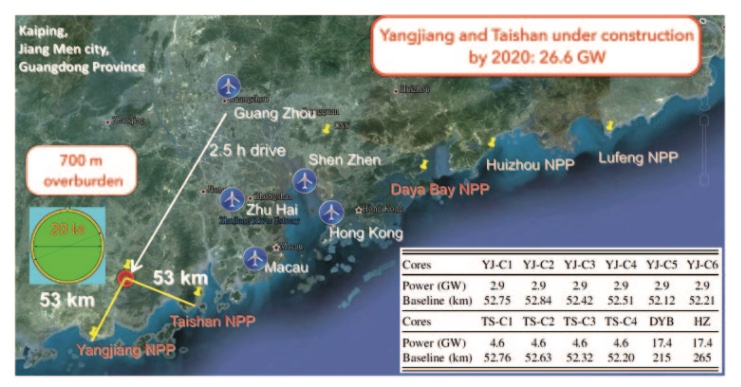
\includegraphics[width=\textwidth]{figures/juno1.jpeg}
    \vspace{2mm}
    \caption{Location of the JUNO site with distances to the nearby reactors, Yangjiang and Taishan at both 53 km as well as Daya Bay at 215 km away.~\cite{75Juno}.}
    \label{fig:juno1}
  \end{minipage}
  \hfill
  \begin{minipage}[b]{0.49\textwidth}
    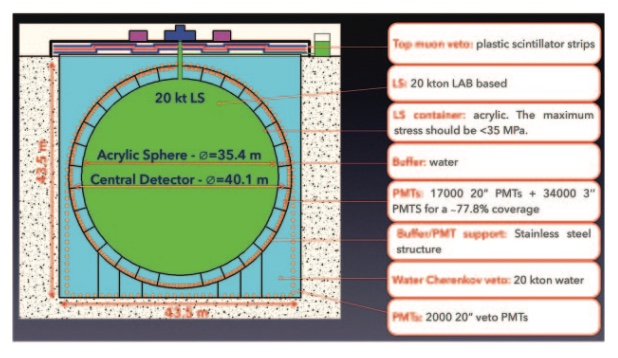
\includegraphics[width=\textwidth]{figures/juno2.jpeg}
       \vspace{2mm}
    \caption{Schematic view of the JUNO detector~\cite{75Juno}.}
     \label{fig:juno2}
  \end{minipage}
\end{figure}

%\pagebreak
\FloatBarrier
\section{Future neutrino oscillation experiments}

\subsection{DUNE}
LBNF/DUNE\cite{23DUNE}, seen in \FigRef{fig:dune2}, is a new experiment currently under construction, with the goal of discovering CP violation in neutrinos with more than 5$\sigma$ sensitivity. DUNE will perform an electron neutrino appearance measurement with a high-powered neutrino beam from Fermilab and a 40 kton liquid argon detector at a distance of 1300 km, in the Homestake mine in South Dakota. A full physics study with its expected performance is presented in~\cite{76Dune}

The main goals are to perform precision measurements of neutrino oscillations to determine $\delta_{CP}$ to $5\sigma$ or better, to determine the neutrino mass ordering, seen in \FigRef{fig:dune1}, and to measure the octant of the mixing angle $\theta_{23}$ all with improved precision.

\begin{figure}[h!]
  \centering
  \begin{minipage}[b]{0.49\textwidth}
    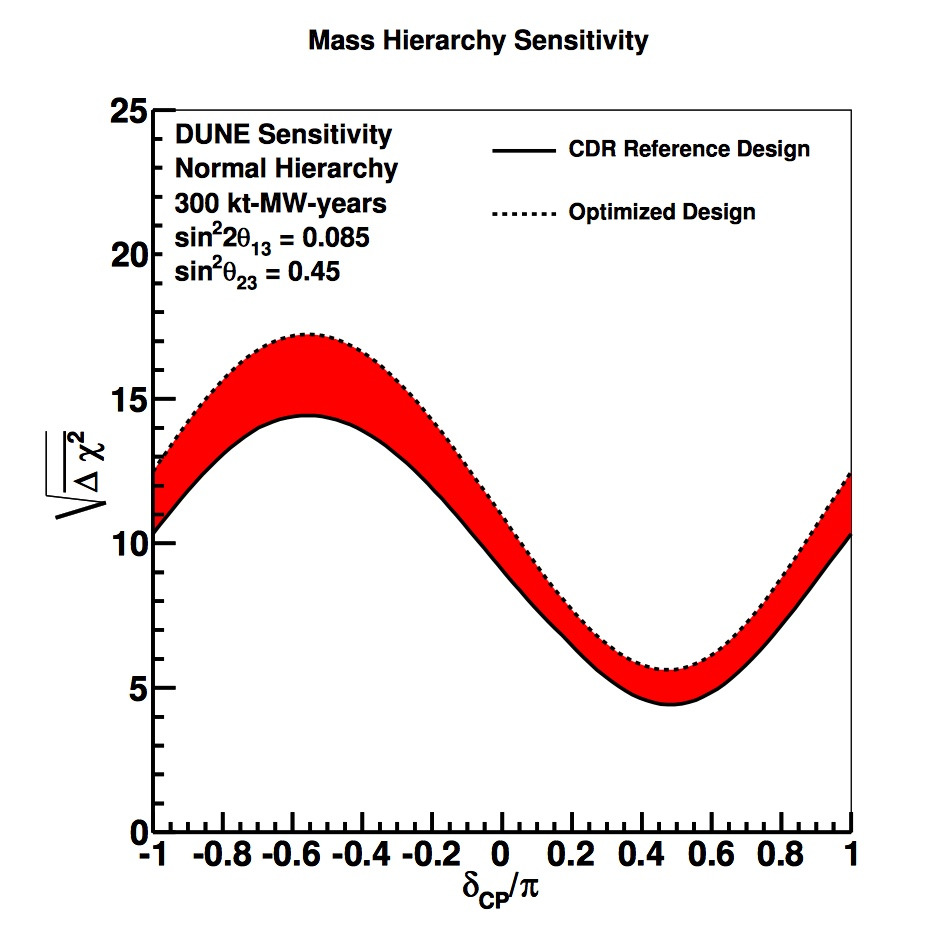
\includegraphics[width=\textwidth]{figures/dune2.jpeg}
    \vspace{2mm}
    \caption{Estimated significance of the mass hierarchy discrimination metric as a function of values for $\delta_{CP}$ ~\cite{23DUNE}.}
    \label{fig:dune1}
  \end{minipage}
  \hfill
  \begin{minipage}[b]{0.49\textwidth}
    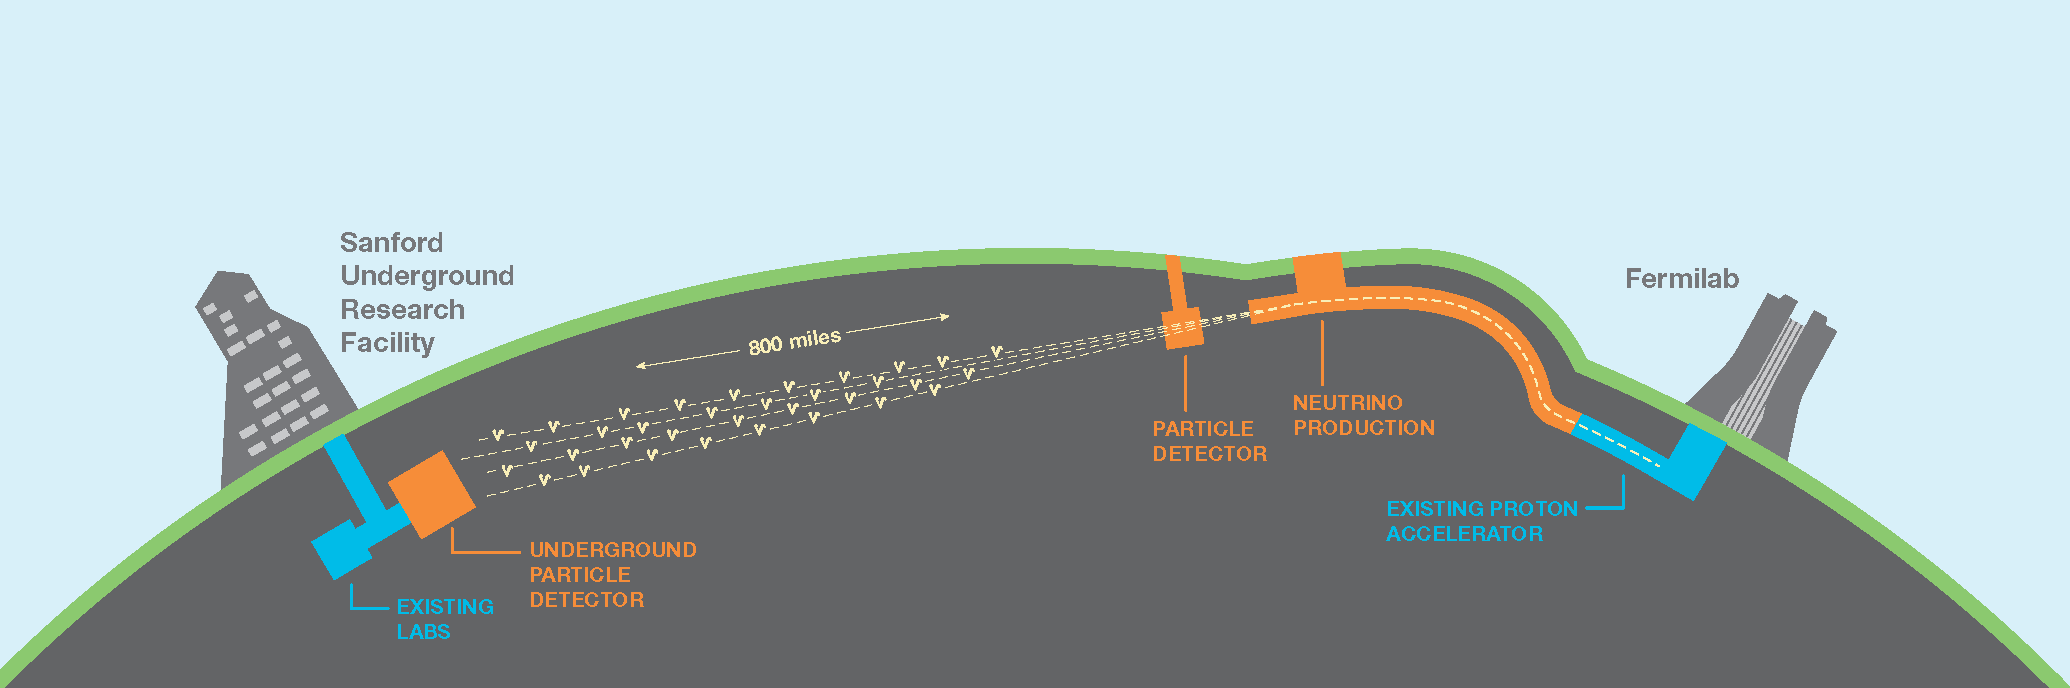
\includegraphics[width=\textwidth]{figures/dune.png}
       \vspace{2mm}
    \caption{Schematic view of the DUNE detectors~\cite{23DUNE}.}
     \label{fig:dune2}
  \end{minipage}
\end{figure}

\subsection{Hyper-K}

The Hyper-Kamiokande Experiment (Hyper-K)~\cite{24HyperK}  builds on the T2K-experiment~\cite{21T2K} by improving the neutrino beam at JPARC, and expanding the water Cherenkov detector by a factor of 10 to a fiducial volume of 500 ktons (figures~\ref{fig:hyper1} and~\ref{fig:hyper2}). Hyper-K aims to improve the sensitivity for $\delta_{CP}$ and to discover CP violation by observing a non-zero value of $\delta_{CP}$ with a sensitivity of 5$\sigma$. It also aims to measure $\Delta \delta < 18^\circ$, determine the mass hierarchy with more than 3$\sigma$ sensitivity and measure $\theta_{23}$ with sufficient accuracy to determine whether it is non-maximal.

%value within $>3\sigma$, and $<18^\circ$ and determine the mass hierarchy within $>3\sigma$ and the sign of $\theta_{23}$ with a $>90\%$ confidence level.

\begin{figure}[h!]
  \centering
  \begin{minipage}[b]{0.59\textwidth}
    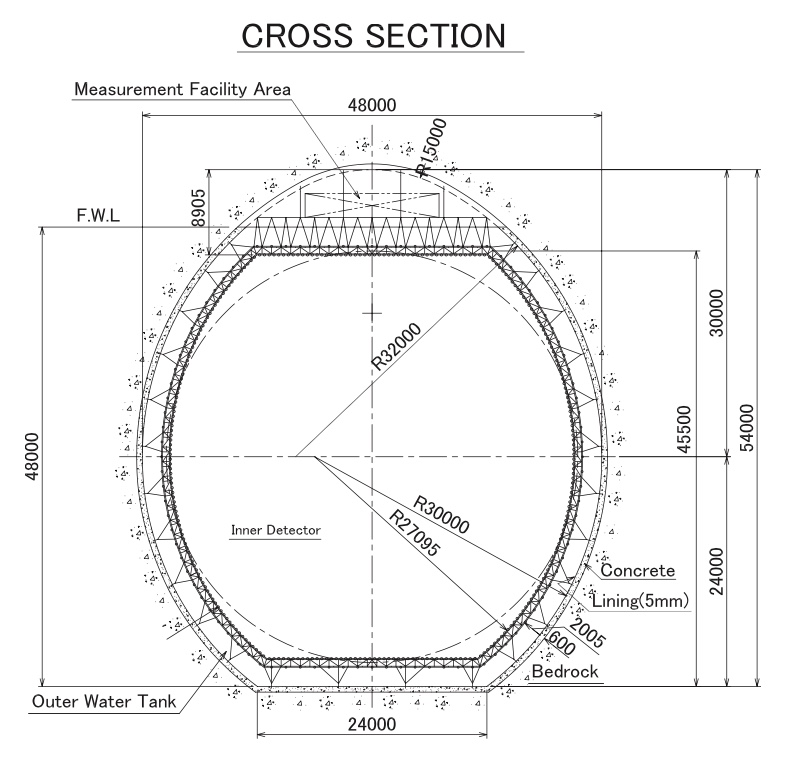
\includegraphics[width=\textwidth]{figures/hyper1.jpeg}
    \vspace{2mm}
    \caption{Cross section view of the Hyper-Kamiokande detector~\cite{24HyperK}.}
    \label{fig:hyper1}
  \end{minipage}
  \hfill
  \begin{minipage}[b]{0.39\textwidth}
    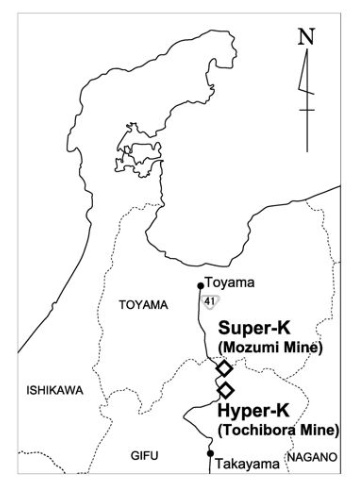
\includegraphics[width=\textwidth]{figures/hyperk2.jpeg}
       \vspace{2mm}
    \caption{A map showing the proposed candidate site~\cite{24HyperK}.}
     \label{fig:hyper2}
  \end{minipage}
\end{figure}

\pagebreak
\FloatBarrier
\section{Neutrino Factory}\label{subsec:nuFACT}
The Neutrino Factory (NuFACT) is a novel concept for a neutrino accelerator which will produce a high-intensity (1000 times higher than previously attained) and a high-energy beam (up to 15 GeV~\cite{Fix7}). Unlike previous experiments it will produce a two flavour, electron and muon, neutrino beam through a muon decay ring. The neutrino factory has the capacity to improve the precision of neutrino oscillation measurements, since the neutrino beam from the decay of muons can be determined with high accuracy. The beam produces one bunch of $\mu^+$ and one bunch of $\mu^-$, so the facility can make measurements of $\nu_{\mu}$ and $\bar{\nu_{e}}$ and $\bar{\nu_{\mu}}$ and $\nu_{e}$ simultaneously. A large 100 kton Magnetised Iron Neutrino Detector (MIND) at a distance of 2000 km is used to perform a measurement of a wrong-sign muon signature that would be the signal for $\nu_e \rightarrow \nu_\mu$ and $\bar{\nu}_e \rightarrow \bar{\nu}_\mu$ oscillations to perform a measurement of $\delta_{CP}$, with an expected accuracy of $\Delta \delta_{CP}\sim 5^\circ$~\cite{25NUfact}. A schematic of the facility is shown in figure \ref{fig:nuFact} showing the full accelerator chain. The full chain starts by producing muons and pions from a proton beam on target. Pions are then captured in a strong solenoid magnetic field surrounding the target. The bunches are sent through the so-called front end containing a phase rotation and an ionisation cooling channel before being re-accelerated to enter the muon storage ring. Before entering the ring the muons are charge separated and go into the storage ring in counter-rotating directions. The muons decay continuously over about 70 turns of the circuit into the following modes with branching ratios:

%The muon beam is then cooled to focus the beam before further accelerating the muon beam to its final energy and introducing it into the decay ring. 

\begin{align}
\mu^- &\rightarrow e^- + \bar{\nu_e} + \nu_\mu, \approx 100\% \\
\mu^- &\rightarrow e^- + \bar{\nu_e} + \nu_\mu + \gamma, <1\% \\
\mu^- &\rightarrow e^- + \bar{\nu_e} + \nu_\mu + e^+ + e^-, <1\% .
\end{align}

The energy spectrum and composition of the neutrino beam is well known as the decays only produce two different neutrino flavours. It is important to note that a $\mu^+$ beam will produce $\bar{\nu}_\mu$ and $\nu_e$ neutrinos and a $\mu^-$ beam will produce $\nu_\mu$ and $\bar{\nu}_e$ neutrinos. Thus for a $\mu^-$ beam any electron neutrinos or muon anti-neutrinos discovered must have been produced through oscillation. To be able to distinguish muons from anti-muons at a detector, a magnetic field is required, motivating the design of any considered detector. Currently there are proposals for NuFACT to be constructed at CERN~\cite{25NUfact}, ESS~\cite{ESS} and FERMILAB~\cite{NuFACTfermi}, where it is also seen as a step toward a full muon collider experiment. The expected precision of $\delta_{CP}$ is shown in \FigRef{fig:nuFactExp}.
%Neutrino factory, explain it. MIND detector for nufact.  MIND needed for charge id, wrong sign muons produced from mu neutrino and anti electron neutrino in accelerator, anti electron to anto muon oscillation. Nufact known 0 anti nu mu in generation, only in oscillation. Prob is 0 for nufact for wrong sign at near detector/source.

\begin{figure}[h!]
\centering
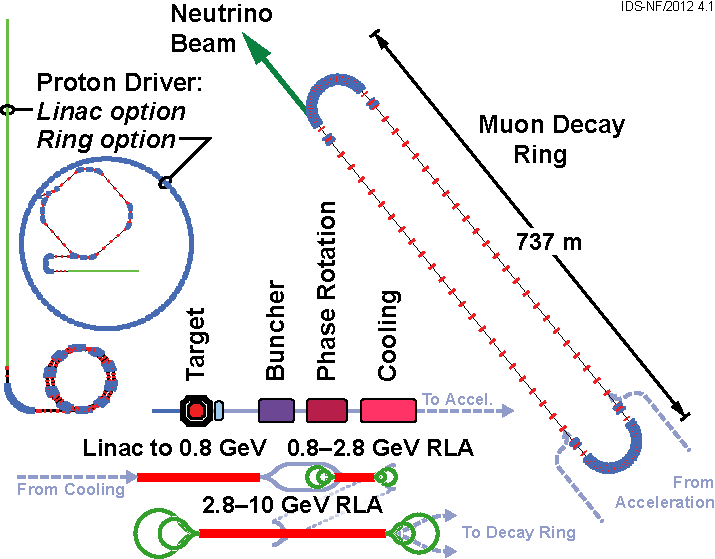
\includegraphics[width=0.9\textwidth]{figures/131112-IDS-NF.pdf}
\caption{Schematic diagram of the Neutrino Factory~\cite{Fix7}.}
\label{fig:nuFact}
\end{figure}

\begin{figure}[h!]
\centering
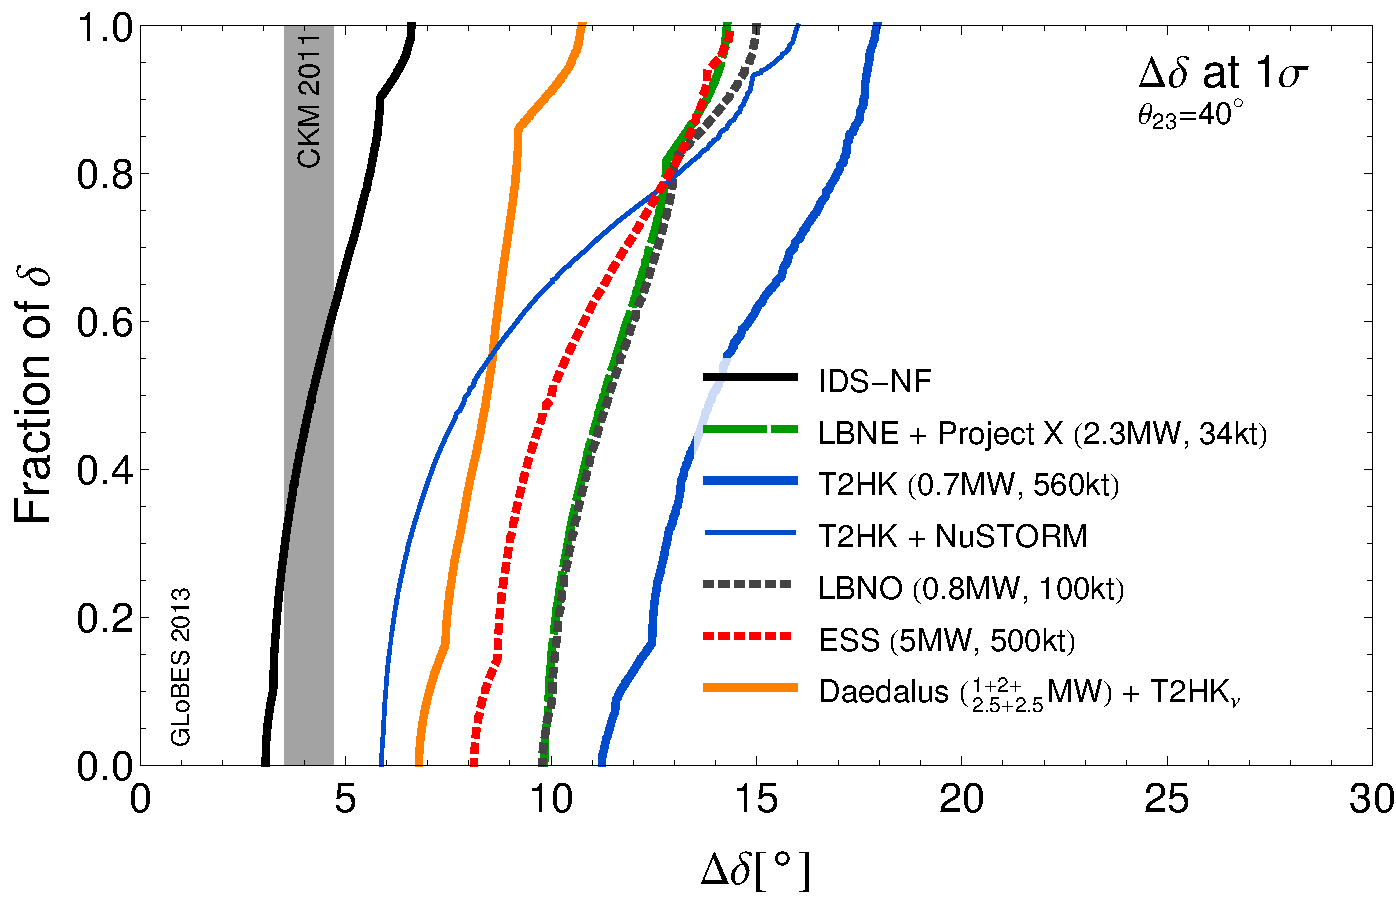
\includegraphics[width=0.9\textwidth]{figures/rdr-cp-precision-comparison-131216.pdf}
\caption{Expected precision for a measurement of the $\delta_{cp}$ at a Neutrino Factory compared to alternate neutrino oscillation facilities~\cite{Fix7}.}
\label{fig:nuFactExp}
\end{figure}


%\textbf{Add in different channels and how it requires a charge identification to be able to identify the various challenge.}

\subsection{NuSTORM}\label{subsec:NuSTORM}

The Neutrino Factory is a complex and expensive facility which requires new technology to be realised. To overcome this, a staged approach has been suggested, where each stage would be delivering physics~\cite{Fix7}. The first stage in this plan is named NuSTORM (Neutrinos from Stored Muons) with a schematic shown in figure~\ref{fig:nuStorm}. The NuSTORM beam is designed to inject 5 GeV/c pions into a muon storage ring, and the ring is designed to store 3.8 GeV/c muons. Compared to the full neutrino factory, NuSTORM is expected to have some pions and kaons for the first pass in the storage ring providing some contamination in the final beam, which can also be used to perform physics measurements, producing both neutrinos and anti-neutrinos for both muon and anti-muon modes and thus a near detector is required to measure the flux of both. 

\begin{figure}[h!]
\centering
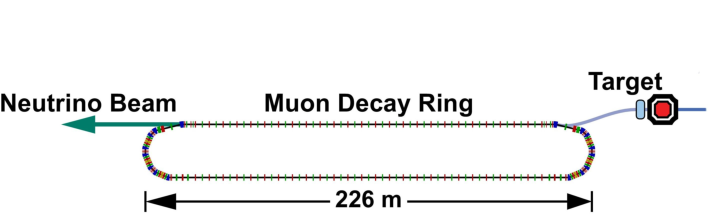
\includegraphics[width=\textwidth]{figures/nuSTORM_schematic.pdf}
\caption{A schematic of a NuSTORM facility~\cite{Fix7}.}
\label{fig:nuStorm}
\end{figure}

For both NuFACT and NuSTORM~\cite{77nustorm} the detector type proposed will be a large Magnetised Iron Neutrino Detector (MIND) type  similar to the ones used in CDHSW~\cite{40CDHSW} and MINOS~\cite{MINOS, NuFACTIDS}. This type of detector, with magnetized steel plates and scintillation plates, is well suited to provide large mass for neutrino experiments and is able to provide momentum measurements by using range and curvature calculations as well as providing charge identification. A MIND type detector has been selected as the baseline detector for a neutrino factory~\cite{ISS, 27Bross} and for NuSTORM, since it is the cheapest and most effective way of producing a large magnetized volume. This has provided the motivation for creating a prototype detector to perform a number of studies.

%\pagebreak
%\subsection{Magnetized Iron Neutrino Detectors}\label{subsec:MINDdetector}
%\textbf{Correct after Pauls comments and add data.}

%Magnetized Iron Neutrino Detectors (MINDs) have been operated in several experiments such as CDHSW~\cite{40CDHSW} and MINOS~\cite{MINOS}. 


%Since water Cherenkov and liquid argon detectors have been established or are actively studied for future very large scale neutrino oscillation experiments, a MIND type detector is not foreseen to be used as the main interaction medium for any planned upcoming experiments.. A MIND type detector can however be used to provide charge identification of muons if positioned downstream of any neutrino target which is not magnetized.

\if{0}
\textbf{OLD}

\subsubsection{IceCube}
The IceCube observatory~\cite{43IceCube} also exploits the fact that particles produced in neutrino interactions emit Cherenkov photons. The low interaction probability of neutrinos require a large interaction volume. The South Pole offers a large interaction volume with very good optical qualities, using this is possible to instrument cubic kilometres of ice with a rather sparse spacing of detectors. The basic detection unit in IceCube is the digital optical module (DOM). The DOM contains, amount other things a PMT encapsulated in a glass pressure sphere to withstand the extreme pressure in the deep ice. In total 5160 DOMS are deployed, instrumenting a volume of one cubic kilometre of ice and allowing detection of astrophysical neutrinos in the energy range of TeV to PeV.

\begin{figure}
\centering
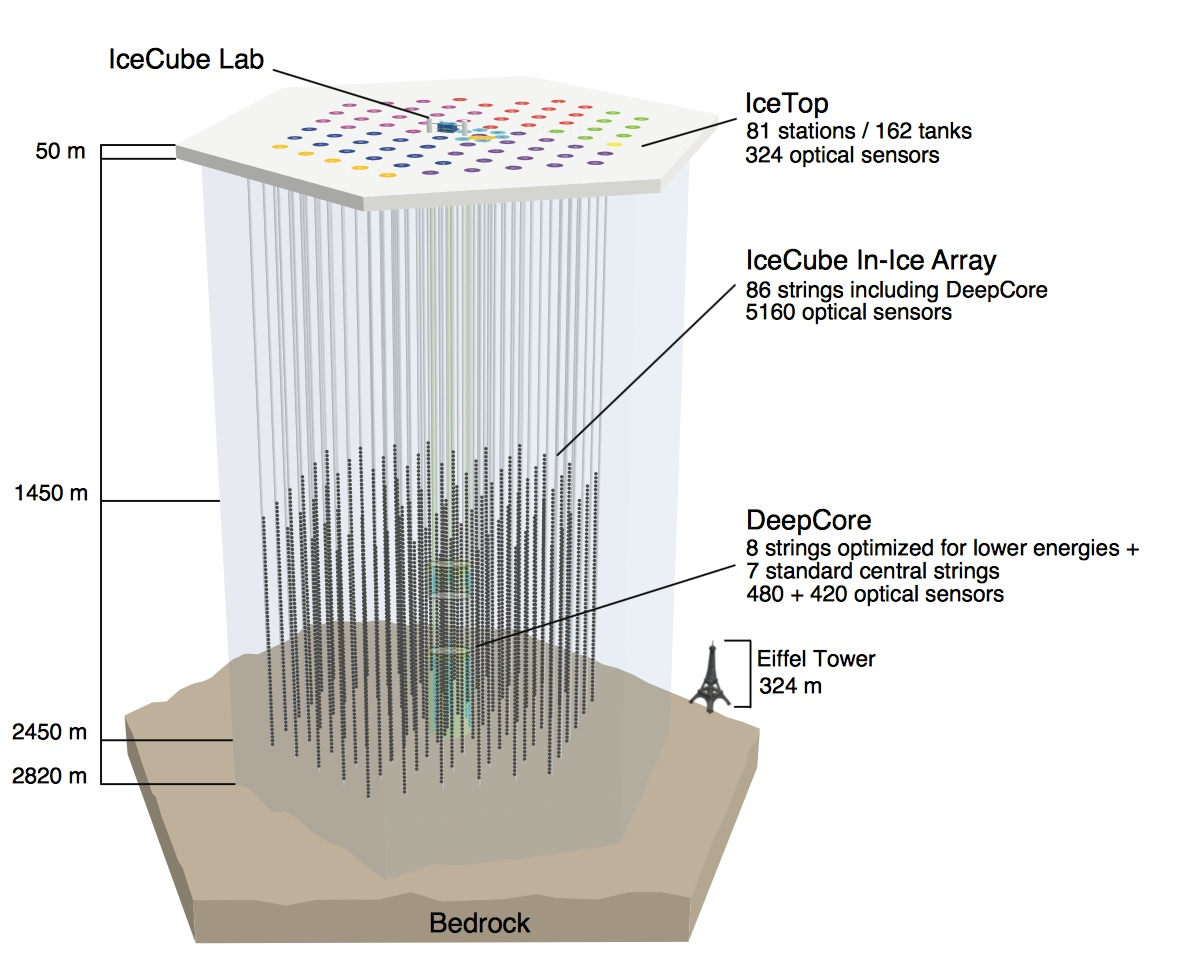
\includegraphics[width=.5\textwidth]{figures/IceCube.jpeg}
\caption{The IceCube Neutrino Observatory}
\end{figure}
\fi

\section{Additional experiments}

There is a lot of interesting physics being performed to understand the parameters of neutrino oscillations as well as also finding a complete theory to describe how neutrinos have mass. Aside from this there are interesting experiments where muon detectors are being used for tomography. One example of this is trying to find chambers in the pyramids which provides a non-intrusive way of searching~\cite{86Morishima}. Another interesting aspect comes from doing precise measurements of nuclear reactors, to be used for non-proliferation~\cite{87Askins} and perhaps even to search for nuclear submarines in a noisy environment where conventional techniques may not work~\cite{88Jocher}.


\section{Summary}
%In this chapter the some history of neutrino experiments have been presented and context given for the Baby MIND experiment.

In this chapter, a history and summary of neutrino experiments measuring neutrino oscillations is presented. These experiments have been able to determine the mixing angle and mass-squared differences of the different eigenstates. Future experiments aim to uncover the remaining questions, such as a measurement of CP violation, the neutrino mass hierarchy between $m_2$ and $m_3$ and whether $\theta_{23}$ is non-maximal. New experiments, such as DUNE and Hyper-K are being planned to make these measurements. Further in the future a neutrino factory could be the ultimate neutrino facility to explore CP violation in the neutrino sector with the best possible accuracy in $\delta_{CP}$. A Magnetised Iron Neutrino Detector (MIND) is required at a neutrino factory, motivating a prototype detector, called Baby MIND. 






%==============================================================================
